\documentclass[twoside]{book}

% Packages required by doxygen
\usepackage{fixltx2e}
\usepackage{calc}
\usepackage{doxygen}
\usepackage[export]{adjustbox} % also loads graphicx
\usepackage{graphicx}
\usepackage[utf8]{inputenc}
\usepackage{makeidx}
\usepackage{multicol}
\usepackage{multirow}
\PassOptionsToPackage{warn}{textcomp}
\usepackage{textcomp}
\usepackage[nointegrals]{wasysym}
\usepackage[table]{xcolor}

% Font selection
\usepackage[T1]{fontenc}
\usepackage[scaled=.90]{helvet}
\usepackage{courier}
\usepackage{amssymb}
\usepackage{sectsty}
\renewcommand{\familydefault}{\sfdefault}
\allsectionsfont{%
  \fontseries{bc}\selectfont%
  \color{darkgray}%
}
\renewcommand{\DoxyLabelFont}{%
  \fontseries{bc}\selectfont%
  \color{darkgray}%
}
\newcommand{\+}{\discretionary{\mbox{\scriptsize$\hookleftarrow$}}{}{}}

% Page & text layout
\usepackage{geometry}
\geometry{%
  a4paper,%
  top=2.5cm,%
  bottom=2.5cm,%
  left=2.5cm,%
  right=2.5cm%
}
\tolerance=750
\hfuzz=15pt
\hbadness=750
\setlength{\emergencystretch}{15pt}
\setlength{\parindent}{0cm}
\setlength{\parskip}{3ex plus 2ex minus 2ex}
\makeatletter
\renewcommand{\paragraph}{%
  \@startsection{paragraph}{4}{0ex}{-1.0ex}{1.0ex}{%
    \normalfont\normalsize\bfseries\SS@parafont%
  }%
}
\renewcommand{\subparagraph}{%
  \@startsection{subparagraph}{5}{0ex}{-1.0ex}{1.0ex}{%
    \normalfont\normalsize\bfseries\SS@subparafont%
  }%
}
\makeatother

% Headers & footers
\usepackage{fancyhdr}
\pagestyle{fancyplain}
\fancyhead[LE]{\fancyplain{}{\bfseries\thepage}}
\fancyhead[CE]{\fancyplain{}{}}
\fancyhead[RE]{\fancyplain{}{\bfseries\leftmark}}
\fancyhead[LO]{\fancyplain{}{\bfseries\rightmark}}
\fancyhead[CO]{\fancyplain{}{}}
\fancyhead[RO]{\fancyplain{}{\bfseries\thepage}}
\fancyfoot[LE]{\fancyplain{}{}}
\fancyfoot[CE]{\fancyplain{}{}}
\fancyfoot[RE]{\fancyplain{}{\bfseries\scriptsize Generated by Doxygen }}
\fancyfoot[LO]{\fancyplain{}{\bfseries\scriptsize Generated by Doxygen }}
\fancyfoot[CO]{\fancyplain{}{}}
\fancyfoot[RO]{\fancyplain{}{}}
\renewcommand{\footrulewidth}{0.4pt}
\renewcommand{\chaptermark}[1]{%
  \markboth{#1}{}%
}
\renewcommand{\sectionmark}[1]{%
  \markright{\thesection\ #1}%
}

% Indices & bibliography
\usepackage{natbib}
\usepackage[titles]{tocloft}
\setcounter{tocdepth}{3}
\setcounter{secnumdepth}{5}
\makeindex

% Hyperlinks (required, but should be loaded last)
\usepackage{ifpdf}
\ifpdf
  \usepackage[pdftex,pagebackref=true]{hyperref}
\else
  \usepackage[ps2pdf,pagebackref=true]{hyperref}
\fi
\hypersetup{%
  colorlinks=true,%
  linkcolor=blue,%
  citecolor=blue,%
  unicode%
}

% Custom commands
\newcommand{\clearemptydoublepage}{%
  \newpage{\pagestyle{empty}\cleardoublepage}%
}

\usepackage{caption}
\captionsetup{labelsep=space,justification=centering,font={bf},singlelinecheck=off,skip=4pt,position=top}

%===== C O N T E N T S =====

\begin{document}

% Titlepage & ToC
\hypersetup{pageanchor=false,
             bookmarksnumbered=true,
             pdfencoding=unicode
            }
\pagenumbering{alph}
\begin{titlepage}
\vspace*{7cm}
\begin{center}%
{\Large Systick Driver \\[1ex]\large Version 1.\+0.\+0 }\\
\vspace*{1cm}
{\large Generated by Doxygen 1.8.13}\\
\end{center}
\end{titlepage}
\clearemptydoublepage
\pagenumbering{roman}
\tableofcontents
\clearemptydoublepage
\pagenumbering{arabic}
\hypersetup{pageanchor=true}

%--- Begin generated contents ---
\chapter{Systick Driver}
\label{md__home_marko__documents_embedded_workspace_systick_driver__r_e_a_d_m_e}
\Hypertarget{md__home_marko__documents_embedded_workspace_systick_driver__r_e_a_d_m_e}
A general wrapper around systick and systick-\/like features to allow for general timekeeping and timeout functionality to other elements of the H\+AL.

\subsection*{Note\+:}

The systick and sysclock elements of the H\+AL are some of the most difficult to use and test, and are generally wrappers around M\+CU vendor created functions, or reimplementations thereof with more freedom (but {\bfseries S\+T\+R\+O\+NG} recommendations). If you have A\+NY doubts about my implementations or experience issues, redirect the interface targets to H\+A\+Ls created by the vendors. 
\chapter{Data Structure Index}
\section{Data Structures}
Here are the data structures with brief descriptions\+:\begin{DoxyCompactList}
\item\contentsline{section}{\hyperlink{structgpio__config__t}{gpio\+\_\+config\+\_\+t} }{\pageref{structgpio__config__t}}{}
\end{DoxyCompactList}

\chapter{File Index}
\section{File List}
Here is a list of all documented files with brief descriptions\+:\begin{DoxyCompactList}
\item\contentsline{section}{\hyperlink{gpio__interface_8h}{gpio\+\_\+interface.\+h} \\*An interface which allows for a level of modularity when using the gpio between different architectures. Usage Notes\+: To port the driver, change the include config line to point instead to the new config.\+h file you want. The config file and the interface file together should provide all definitions to implement what you need in the machine specific c implementation file }{\pageref{gpio__interface_8h}}{}
\item\contentsline{section}{\hyperlink{gpio__stm32f411_8c}{gpio\+\_\+stm32f411.\+c} \\*Machine specific implementation of gpio }{\pageref{gpio__stm32f411_8c}}{}
\item\contentsline{section}{\hyperlink{gpio__stm32f411__config_8c}{gpio\+\_\+stm32f411\+\_\+config.\+c} \\*A file defining a config table which contains all information required by gpio\+\_\+init to initialise the pins with the desired behaviour }{\pageref{gpio__stm32f411__config_8c}}{}
\item\contentsline{section}{\hyperlink{gpio__stm32f411__config_8h}{gpio\+\_\+stm32f411\+\_\+config.\+h} \\*Machine specific configuration enumerations and structures }{\pageref{gpio__stm32f411__config_8h}}{}
\end{DoxyCompactList}

\chapter{Data Structure Documentation}
\hypertarget{structsystick__config__t}{}\section{systick\+\_\+config\+\_\+t Struct Reference}
\label{structsystick__config__t}\index{systick\+\_\+config\+\_\+t@{systick\+\_\+config\+\_\+t}}


{\ttfamily \#include $<$systick\+\_\+stm32f411\+\_\+config.\+h$>$}

\subsection*{Data Fields}
\begin{DoxyCompactItemize}
\item 
\hyperlink{systick__stm32f411__config_8h_a54abff3d12292257e357d04094ebc415}{systick\+\_\+enabled\+\_\+t} \hyperlink{structsystick__config__t_a072e52389584956edd057c591c1c7cd8}{enable\+\_\+systick}
\item 
uint32\+\_\+t \hyperlink{structsystick__config__t_a5d1767c41ce5e869439e7197fd6a7373}{tick\+\_\+freq\+\_\+khz}
\item 
\hyperlink{systick__stm32f411__config_8h_a82589cfda6cc55b21d80e5e3f47b69d9}{systick\+\_\+interrupt\+\_\+t} \hyperlink{structsystick__config__t_ae4174393003a47f219770a2e5793de45}{enable\+\_\+systick\+\_\+interrupt}
\item 
\hyperlink{systick__stm32f411__config_8h_a39469603d3120252cd4f82defbd9525e}{systick\+\_\+clock\+\_\+source\+\_\+t} \hyperlink{structsystick__config__t_a47a24c541e5d6123ec5825484d4f85f0}{clock\+\_\+source}
\end{DoxyCompactItemize}


\subsection{Detailed Description}
Struct containing relevant configuration data to enable the systick 

\subsection{Field Documentation}
\mbox{\Hypertarget{structsystick__config__t_a47a24c541e5d6123ec5825484d4f85f0}\label{structsystick__config__t_a47a24c541e5d6123ec5825484d4f85f0}} 
\index{systick\+\_\+config\+\_\+t@{systick\+\_\+config\+\_\+t}!clock\+\_\+source@{clock\+\_\+source}}
\index{clock\+\_\+source@{clock\+\_\+source}!systick\+\_\+config\+\_\+t@{systick\+\_\+config\+\_\+t}}
\subsubsection{\texorpdfstring{clock\+\_\+source}{clock\_source}}
{\footnotesize\ttfamily \hyperlink{systick__stm32f411__config_8h_a39469603d3120252cd4f82defbd9525e}{systick\+\_\+clock\+\_\+source\+\_\+t} clock\+\_\+source}

The systick clock source. Recommended value is S\+Y\+S\+T\+I\+C\+K\+\_\+\+I\+N\+T\+E\+R\+N\+A\+L\+\_\+\+C\+L\+O\+CK \mbox{\Hypertarget{structsystick__config__t_a072e52389584956edd057c591c1c7cd8}\label{structsystick__config__t_a072e52389584956edd057c591c1c7cd8}} 
\index{systick\+\_\+config\+\_\+t@{systick\+\_\+config\+\_\+t}!enable\+\_\+systick@{enable\+\_\+systick}}
\index{enable\+\_\+systick@{enable\+\_\+systick}!systick\+\_\+config\+\_\+t@{systick\+\_\+config\+\_\+t}}
\subsubsection{\texorpdfstring{enable\+\_\+systick}{enable\_systick}}
{\footnotesize\ttfamily \hyperlink{systick__stm32f411__config_8h_a54abff3d12292257e357d04094ebc415}{systick\+\_\+enabled\+\_\+t} enable\+\_\+systick}

Whether or not the systick should be enabled. Recommended value is S\+Y\+S\+T\+I\+C\+K\+\_\+\+E\+N\+A\+B\+L\+ED \mbox{\Hypertarget{structsystick__config__t_ae4174393003a47f219770a2e5793de45}\label{structsystick__config__t_ae4174393003a47f219770a2e5793de45}} 
\index{systick\+\_\+config\+\_\+t@{systick\+\_\+config\+\_\+t}!enable\+\_\+systick\+\_\+interrupt@{enable\+\_\+systick\+\_\+interrupt}}
\index{enable\+\_\+systick\+\_\+interrupt@{enable\+\_\+systick\+\_\+interrupt}!systick\+\_\+config\+\_\+t@{systick\+\_\+config\+\_\+t}}
\subsubsection{\texorpdfstring{enable\+\_\+systick\+\_\+interrupt}{enable\_systick\_interrupt}}
{\footnotesize\ttfamily \hyperlink{systick__stm32f411__config_8h_a82589cfda6cc55b21d80e5e3f47b69d9}{systick\+\_\+interrupt\+\_\+t} enable\+\_\+systick\+\_\+interrupt}

Whether or not the systick interrupt should be enabled. Recommended value si S\+Y\+S\+T\+I\+C\+K\+\_\+\+I\+N\+T\+\_\+\+E\+N\+A\+B\+L\+ED. \mbox{\Hypertarget{structsystick__config__t_a5d1767c41ce5e869439e7197fd6a7373}\label{structsystick__config__t_a5d1767c41ce5e869439e7197fd6a7373}} 
\index{systick\+\_\+config\+\_\+t@{systick\+\_\+config\+\_\+t}!tick\+\_\+freq\+\_\+khz@{tick\+\_\+freq\+\_\+khz}}
\index{tick\+\_\+freq\+\_\+khz@{tick\+\_\+freq\+\_\+khz}!systick\+\_\+config\+\_\+t@{systick\+\_\+config\+\_\+t}}
\subsubsection{\texorpdfstring{tick\+\_\+freq\+\_\+khz}{tick\_freq\_khz}}
{\footnotesize\ttfamily uint32\+\_\+t tick\+\_\+freq\+\_\+khz}

How quickly the systick should trigger in k\+Hz. Recommended value is 1 

The documentation for this struct was generated from the following file\+:\begin{DoxyCompactItemize}
\item 
/home/marko/\+Documents/embedded\+\_\+workspace/systick\+\_\+driver/\hyperlink{systick__stm32f411__config_8h}{systick\+\_\+stm32f411\+\_\+config.\+h}\end{DoxyCompactItemize}

\chapter{File Documentation}
\hypertarget{systick__interface_8h}{}\section{/home/marko/\+Documents/embedded\+\_\+workspace/systick\+\_\+driver/systick\+\_\+interface.h File Reference}
\label{systick__interface_8h}\index{/home/marko/\+Documents/embedded\+\_\+workspace/systick\+\_\+driver/systick\+\_\+interface.\+h@{/home/marko/\+Documents/embedded\+\_\+workspace/systick\+\_\+driver/systick\+\_\+interface.\+h}}


General interface covering user accesses to initialise the system wide tick for timeout/timekeeping operations.  


{\ttfamily \#include \char`\"{}systick\+\_\+stm32f411\+\_\+config.\+h\char`\"{}}\newline
Include dependency graph for systick\+\_\+interface.\+h\+:\nopagebreak
\begin{figure}[H]
\begin{center}
\leavevmode
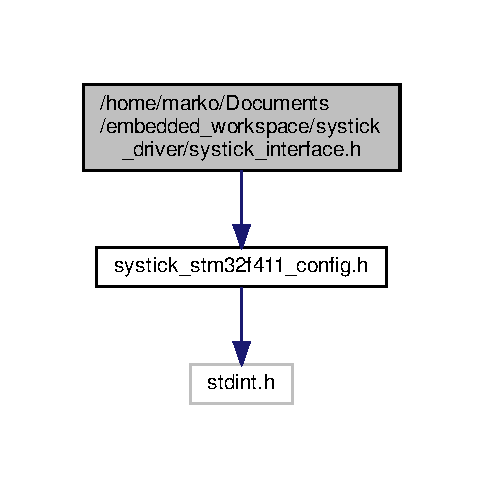
\includegraphics[width=232pt]{systick__interface_8h__incl}
\end{center}
\end{figure}
This graph shows which files directly or indirectly include this file\+:\nopagebreak
\begin{figure}[H]
\begin{center}
\leavevmode
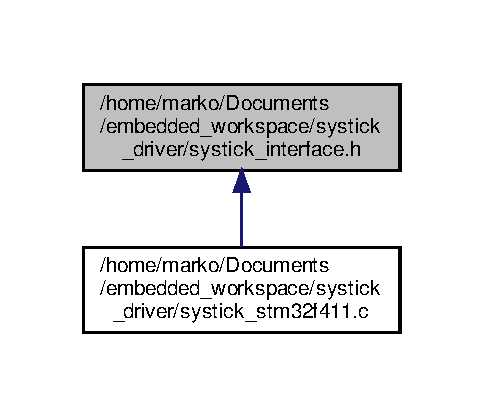
\includegraphics[width=232pt]{systick__interface_8h__dep__incl}
\end{center}
\end{figure}
\subsection*{Typedefs}
\begin{DoxyCompactItemize}
\item 
typedef void($\ast$ \hyperlink{systick__interface_8h_a90b4dba6415b72ebd50fc0540dcd2ddf}{systick\+\_\+callback\+\_\+t}) (void)
\end{DoxyCompactItemize}
\subsection*{Functions}
\begin{DoxyCompactItemize}
\item 
void \hyperlink{systick__interface_8h_a05307f714c3701c4b6b396a833f39e92}{systick\+\_\+init} (\hyperlink{structsystick__config__t}{systick\+\_\+config\+\_\+t} $\ast$config)
\item 
void \hyperlink{systick__interface_8h_a6fb10375fe1f7fbef5bdbe3ab33a5376}{systick\+\_\+tick\+\_\+freq\+\_\+set} (\hyperlink{structsystick__config__t}{systick\+\_\+config\+\_\+t} $\ast$config)
\item 
void \hyperlink{systick__interface_8h_a618b49039ac69306cc271b98af1fb935}{systick\+\_\+interrupt\+\_\+control} (\hyperlink{systick__stm32f411__config_8h_a82589cfda6cc55b21d80e5e3f47b69d9}{systick\+\_\+interrupt\+\_\+t} interrupt\+\_\+control)
\item 
void \hyperlink{systick__interface_8h_ab315ae133959817580ef089539a7ea3f}{systick\+\_\+pause} (void)
\item 
void \hyperlink{systick__interface_8h_abd308166607c7424fb1ae67fb24cba5e}{systick\+\_\+resume} (void)
\item 
uint32\+\_\+t \hyperlink{systick__interface_8h_afdf1221fe41470afc9faf278a871b68c}{systick\+\_\+get\+\_\+tick} (void)
\item 
void \hyperlink{systick__interface_8h_ab0275b71c7f7a9080dcac8ffc68559c7}{systick\+\_\+delay} (uint32\+\_\+t delay\+\_\+ms)
\item 
void \hyperlink{systick__interface_8h_a97fc9935ef263cd958116a6ecdfd835f}{systick\+\_\+increment} (void)
\item 
void \hyperlink{systick__interface_8h_a70216cf1d168d9c2239c87878745a631}{systick\+\_\+callback\+\_\+register} (\hyperlink{systick__interface_8h_a90b4dba6415b72ebd50fc0540dcd2ddf}{systick\+\_\+callback\+\_\+t} callback\+\_\+func)
\item 
void \hyperlink{systick__interface_8h_a8e3818296c4ed279cc0f2967bcdddcee}{systick\+\_\+irq\+\_\+handler} (void)
\end{DoxyCompactItemize}


\subsection{Detailed Description}
General interface covering user accesses to initialise the system wide tick for timeout/timekeeping operations. 



\subsection{Typedef Documentation}
\mbox{\Hypertarget{systick__interface_8h_a90b4dba6415b72ebd50fc0540dcd2ddf}\label{systick__interface_8h_a90b4dba6415b72ebd50fc0540dcd2ddf}} 
\index{systick\+\_\+interface.\+h@{systick\+\_\+interface.\+h}!systick\+\_\+callback\+\_\+t@{systick\+\_\+callback\+\_\+t}}
\index{systick\+\_\+callback\+\_\+t@{systick\+\_\+callback\+\_\+t}!systick\+\_\+interface.\+h@{systick\+\_\+interface.\+h}}
\subsubsection{\texorpdfstring{systick\+\_\+callback\+\_\+t}{systick\_callback\_t}}
{\footnotesize\ttfamily typedef void($\ast$ systick\+\_\+callback\+\_\+t) (void)}

Systick callback type used to send interrupt behaviour functions to the irq handler 

\subsection{Function Documentation}
\mbox{\Hypertarget{systick__interface_8h_a70216cf1d168d9c2239c87878745a631}\label{systick__interface_8h_a70216cf1d168d9c2239c87878745a631}} 
\index{systick\+\_\+interface.\+h@{systick\+\_\+interface.\+h}!systick\+\_\+callback\+\_\+register@{systick\+\_\+callback\+\_\+register}}
\index{systick\+\_\+callback\+\_\+register@{systick\+\_\+callback\+\_\+register}!systick\+\_\+interface.\+h@{systick\+\_\+interface.\+h}}
\subsubsection{\texorpdfstring{systick\+\_\+callback\+\_\+register()}{systick\_callback\_register()}}
{\footnotesize\ttfamily void systick\+\_\+callback\+\_\+register (\begin{DoxyParamCaption}\item[{\hyperlink{systick__interface_8h_a90b4dba6415b72ebd50fc0540dcd2ddf}{systick\+\_\+callback\+\_\+t}}]{callback\+\_\+func }\end{DoxyParamCaption})}

{\bfseries Description\+:} \begin{DoxyVerb}Registers the callback function as the desired on-interrupt functionality.
\end{DoxyVerb}


P\+R\+E-\/\+C\+O\+N\+D\+I\+T\+I\+ON\+: None.

P\+O\+S\+T-\/\+C\+O\+N\+D\+I\+T\+I\+ON\+: the systick\+\_\+callback function pointer variable now points to the desired function


\begin{DoxyParams}{Parameters}
{\em callback\+\_\+func} & a function pointer to a void ($\ast$function)(void) \\
\hline
\end{DoxyParams}
\begin{DoxyReturn}{Returns}
void
\end{DoxyReturn}
{\bfseries Example\+:} 
\begin{DoxyCode}
\hyperlink{systick__interface_8h_a70216cf1d168d9c2239c87878745a631}{systick\_callback\_register}(&interrupt\_behaviour);

\textcolor{comment}{//the irq handler will now call interrupt\_behaviour}
  SysTick\_IRQHandler(\textcolor{keywordtype}{void})
  \{
      \hyperlink{systick__interface_8h_a8e3818296c4ed279cc0f2967bcdddcee}{systick\_irq\_handler}();
  \}
\end{DoxyCode}


\begin{DoxySeeAlso}{See also}
\hyperlink{systick__stm32f411_8c_a8e3818296c4ed279cc0f2967bcdddcee}{systick\+\_\+irq\+\_\+handler}
\end{DoxySeeAlso}
~\newline
{\bfseries  -\/ C\+H\+A\+N\+GE H\+I\+S\+T\+O\+RY -\/ }

\tabulinesep=1mm
\begin{longtabu} spread 0pt [c]{*{4}{|X[-1]}|}
\hline
Date &Software Version &Initials &Description  \\\cline{1-4}
\end{longtabu}
~\newline
~\newline
 

 \mbox{\Hypertarget{systick__interface_8h_ab0275b71c7f7a9080dcac8ffc68559c7}\label{systick__interface_8h_ab0275b71c7f7a9080dcac8ffc68559c7}} 
\index{systick\+\_\+interface.\+h@{systick\+\_\+interface.\+h}!systick\+\_\+delay@{systick\+\_\+delay}}
\index{systick\+\_\+delay@{systick\+\_\+delay}!systick\+\_\+interface.\+h@{systick\+\_\+interface.\+h}}
\subsubsection{\texorpdfstring{systick\+\_\+delay()}{systick\_delay()}}
{\footnotesize\ttfamily void systick\+\_\+delay (\begin{DoxyParamCaption}\item[{uint32\+\_\+t}]{delay\+\_\+ms }\end{DoxyParamCaption})}

{\bfseries Description\+:} \begin{DoxyVerb}Delays the program for the duration of delay_ms in milliseconds
\end{DoxyVerb}


P\+R\+E-\/\+C\+O\+N\+D\+I\+T\+I\+ON\+: None

P\+O\+S\+T-\/\+C\+O\+N\+D\+I\+T\+I\+ON\+: delay\+\_\+ms have gone by and the rest of the program will resume


\begin{DoxyParams}{Parameters}
{\em delay\+\_\+ms} & is the length of time the user wishes to way\\
\hline
\end{DoxyParams}
\begin{DoxyReturn}{Returns}
void
\end{DoxyReturn}
{\bfseries Example\+:} 


\begin{DoxyCode}
\hyperlink{systick__interface_8h_ab0275b71c7f7a9080dcac8ffc68559c7}{systick\_delay}(200);
\end{DoxyCode}


\begin{DoxySeeAlso}{See also}
\hyperlink{systick__stm32f411_8c_a6fb10375fe1f7fbef5bdbe3ab33a5376}{systick\+\_\+tick\+\_\+freq\+\_\+set} 

\hyperlink{systick__stm32f411_8c_afdf1221fe41470afc9faf278a871b68c}{systick\+\_\+get\+\_\+tick}
\end{DoxySeeAlso}
~\newline
{\bfseries  -\/ C\+H\+A\+N\+GE H\+I\+S\+T\+O\+RY -\/ }

\tabulinesep=1mm
\begin{longtabu} spread 0pt [c]{*{4}{|X[-1]}|}
\hline
Date &Software Version &Initials &Description  \\\cline{1-4}
\end{longtabu}
~\newline
~\newline
 

 \mbox{\Hypertarget{systick__interface_8h_afdf1221fe41470afc9faf278a871b68c}\label{systick__interface_8h_afdf1221fe41470afc9faf278a871b68c}} 
\index{systick\+\_\+interface.\+h@{systick\+\_\+interface.\+h}!systick\+\_\+get\+\_\+tick@{systick\+\_\+get\+\_\+tick}}
\index{systick\+\_\+get\+\_\+tick@{systick\+\_\+get\+\_\+tick}!systick\+\_\+interface.\+h@{systick\+\_\+interface.\+h}}
\subsubsection{\texorpdfstring{systick\+\_\+get\+\_\+tick()}{systick\_get\_tick()}}
{\footnotesize\ttfamily uint32\+\_\+t systick\+\_\+get\+\_\+tick (\begin{DoxyParamCaption}\item[{void}]{ }\end{DoxyParamCaption})}

{\bfseries Description\+:} \begin{DoxyVerb}DReturns the current value of the tick_ms variable
\end{DoxyVerb}


P\+R\+E-\/\+C\+O\+N\+D\+I\+T\+I\+ON\+: None

P\+O\+S\+T-\/\+C\+O\+N\+D\+I\+T\+I\+ON\+: The function has returned the current value of the tick variable.

\begin{DoxyReturn}{Returns}
uint32\+\_\+t the current tick value
\end{DoxyReturn}
{\bfseries Example\+:} 


\begin{DoxyCode}
uint32\_t current\_tick = \hyperlink{systick__interface_8h_afdf1221fe41470afc9faf278a871b68c}{systick\_get\_tick}();
\end{DoxyCode}


\begin{DoxySeeAlso}{See also}
\hyperlink{systick__stm32f411_8c_a6fb10375fe1f7fbef5bdbe3ab33a5376}{systick\+\_\+tick\+\_\+freq\+\_\+set} 

\hyperlink{systick__stm32f411_8c_ab0275b71c7f7a9080dcac8ffc68559c7}{systick\+\_\+delay}
\end{DoxySeeAlso}
~\newline
{\bfseries  -\/ C\+H\+A\+N\+GE H\+I\+S\+T\+O\+RY -\/ }

\tabulinesep=1mm
\begin{longtabu} spread 0pt [c]{*{4}{|X[-1]}|}
\hline
Date &Software Version &Initials &Description  \\\cline{1-4}
\end{longtabu}
~\newline
~\newline
 

 \mbox{\Hypertarget{systick__interface_8h_a97fc9935ef263cd958116a6ecdfd835f}\label{systick__interface_8h_a97fc9935ef263cd958116a6ecdfd835f}} 
\index{systick\+\_\+interface.\+h@{systick\+\_\+interface.\+h}!systick\+\_\+increment@{systick\+\_\+increment}}
\index{systick\+\_\+increment@{systick\+\_\+increment}!systick\+\_\+interface.\+h@{systick\+\_\+interface.\+h}}
\subsubsection{\texorpdfstring{systick\+\_\+increment()}{systick\_increment()}}
{\footnotesize\ttfamily void systick\+\_\+increment (\begin{DoxyParamCaption}\item[{void}]{ }\end{DoxyParamCaption})}

{\bfseries Description\+:} \begin{DoxyVerb}Increments the tick by the number of milliseconds between systick register
overflows. Called within systick_irq_handler.
\end{DoxyVerb}


P\+R\+E-\/\+C\+O\+N\+D\+I\+T\+I\+ON\+: None.

P\+O\+S\+T-\/\+C\+O\+N\+D\+I\+T\+I\+ON\+: tick\+\_\+ms has incremented by tick\+\_\+freq milliseconds

\begin{DoxyReturn}{Returns}
void
\end{DoxyReturn}
{\bfseries Example\+:} 
\begin{DoxyCode}
\textcolor{comment}{//By default is called automatically upon SysTick interrupt}
  SysTick\_IRQHandler(\textcolor{keywordtype}{void})
  \{
      \hyperlink{systick__interface_8h_a8e3818296c4ed279cc0f2967bcdddcee}{systick\_irq\_handler}();
  \}
\end{DoxyCode}


\begin{DoxySeeAlso}{See also}
\hyperlink{systick__stm32f411_8c_a70216cf1d168d9c2239c87878745a631}{systick\+\_\+callback\+\_\+register} 

\hyperlink{systick__stm32f411_8c_a8e3818296c4ed279cc0f2967bcdddcee}{systick\+\_\+irq\+\_\+handler}
\end{DoxySeeAlso}
~\newline
{\bfseries  -\/ C\+H\+A\+N\+GE H\+I\+S\+T\+O\+RY -\/ }

\tabulinesep=1mm
\begin{longtabu} spread 0pt [c]{*{4}{|X[-1]}|}
\hline
Date &Software Version &Initials &Description  \\\cline{1-4}
\end{longtabu}
~\newline
~\newline
 

 \mbox{\Hypertarget{systick__interface_8h_a05307f714c3701c4b6b396a833f39e92}\label{systick__interface_8h_a05307f714c3701c4b6b396a833f39e92}} 
\index{systick\+\_\+interface.\+h@{systick\+\_\+interface.\+h}!systick\+\_\+init@{systick\+\_\+init}}
\index{systick\+\_\+init@{systick\+\_\+init}!systick\+\_\+interface.\+h@{systick\+\_\+interface.\+h}}
\subsubsection{\texorpdfstring{systick\+\_\+init()}{systick\_init()}}
{\footnotesize\ttfamily void systick\+\_\+init (\begin{DoxyParamCaption}\item[{\hyperlink{structsystick__config__t}{systick\+\_\+config\+\_\+t} $\ast$}]{config }\end{DoxyParamCaption})}

{\bfseries Description\+:} \begin{DoxyVerb}Carries out the initialisation of the the systick based on information in the
config table
\end{DoxyVerb}


P\+R\+E-\/\+C\+O\+N\+D\+I\+T\+I\+ON\+: The clock system (R\+CC) has been initialised. P\+R\+E-\/\+C\+O\+N\+D\+I\+T\+I\+ON\+: The desired frequency (tick\+\_\+freq\+\_\+khz) results in a number small enough to fit the 0x\+F\+F\+F\+F\+FF mask P\+R\+E-\/\+C\+O\+N\+D\+I\+T\+I\+ON\+: (Soft Assert) the systick is enabled through its config register

P\+O\+S\+T-\/\+C\+O\+N\+D\+I\+T\+I\+ON\+: The systick has been configured to count with the desired frequency P\+O\+S\+T-\/\+C\+O\+N\+D\+I\+T\+I\+ON\+: The systick interrupt has been enabled (if desired) and its priority set to maximum. P\+O\+S\+T-\/\+C\+O\+N\+D\+I\+T\+I\+ON\+: The systick clock source has been set to the desired option


\begin{DoxyParams}{Parameters}
{\em config} & a pointer to the systick configuration structure\\
\hline
\end{DoxyParams}
\begin{DoxyReturn}{Returns}
void
\end{DoxyReturn}
{\bfseries Example\+:} 


\begin{DoxyCode}
\hyperlink{structsystick__config__t}{systick\_config\_t} *tick\_config = \hyperlink{systick__stm32f411__config_8c_a736aba702662d732de33f92b1fef7ad0}{systick\_config\_get}();
\hyperlink{systick__interface_8h_a05307f714c3701c4b6b396a833f39e92}{systick\_init}(tick\_config);
\end{DoxyCode}


\begin{DoxySeeAlso}{See also}
\hyperlink{systick__stm32f411__config_8h_a736aba702662d732de33f92b1fef7ad0}{systick\+\_\+config\+\_\+get} 

\hyperlink{systick__stm32f411_8c_a6fb10375fe1f7fbef5bdbe3ab33a5376}{systick\+\_\+tick\+\_\+freq\+\_\+set} 

\hyperlink{systick__stm32f411_8c_ab315ae133959817580ef089539a7ea3f}{systick\+\_\+pause} 

\hyperlink{systick__stm32f411_8c_abd308166607c7424fb1ae67fb24cba5e}{systick\+\_\+resume} 

\hyperlink{systick__stm32f411_8c_a618b49039ac69306cc271b98af1fb935}{systick\+\_\+interrupt\+\_\+control} ~\newline
{\bfseries  -\/ C\+H\+A\+N\+GE H\+I\+S\+T\+O\+RY -\/ }
\end{DoxySeeAlso}
\tabulinesep=1mm
\begin{longtabu} spread 0pt [c]{*{4}{|X[-1]}|}
\hline
Date &Software Version &Initials &Description  \\\cline{1-4}
\end{longtabu}
~\newline
~\newline
 

 \mbox{\Hypertarget{systick__interface_8h_a618b49039ac69306cc271b98af1fb935}\label{systick__interface_8h_a618b49039ac69306cc271b98af1fb935}} 
\index{systick\+\_\+interface.\+h@{systick\+\_\+interface.\+h}!systick\+\_\+interrupt\+\_\+control@{systick\+\_\+interrupt\+\_\+control}}
\index{systick\+\_\+interrupt\+\_\+control@{systick\+\_\+interrupt\+\_\+control}!systick\+\_\+interface.\+h@{systick\+\_\+interface.\+h}}
\subsubsection{\texorpdfstring{systick\+\_\+interrupt\+\_\+control()}{systick\_interrupt\_control()}}
{\footnotesize\ttfamily void systick\+\_\+interrupt\+\_\+control (\begin{DoxyParamCaption}\item[{\hyperlink{systick__stm32f411__config_8h_a82589cfda6cc55b21d80e5e3f47b69d9}{systick\+\_\+interrupt\+\_\+t}}]{interrupt\+\_\+control }\end{DoxyParamCaption})}

{\bfseries Description\+:} \begin{DoxyVerb}Enables or disables the systick interrupt
\end{DoxyVerb}


P\+R\+E-\/\+C\+O\+N\+D\+I\+T\+I\+ON\+: (Soft Assert) The systick is paused

P\+O\+S\+T-\/\+C\+O\+N\+D\+I\+T\+I\+ON\+: The systick interrupt is enabled or disabled, as per the input


\begin{DoxyParams}{Parameters}
{\em interrupt\+\_\+control} & Control parameter defining if the interrupt will be activated or deactivated \\
\hline
\end{DoxyParams}
\begin{DoxyReturn}{Returns}
void
\end{DoxyReturn}
{\bfseries Example\+:} 


\begin{DoxyCode}
\hyperlink{systick__interface_8h_ab315ae133959817580ef089539a7ea3f}{systick\_pause}();
\hyperlink{systick__interface_8h_a618b49039ac69306cc271b98af1fb935}{systick\_interrupt\_control}(SYSTICK\_INT\_ENABLED);
\hyperlink{systick__interface_8h_abd308166607c7424fb1ae67fb24cba5e}{systick\_resume}();
\end{DoxyCode}


\begin{DoxySeeAlso}{See also}
\hyperlink{systick__stm32f411_8c_a05307f714c3701c4b6b396a833f39e92}{systick\+\_\+init} 

\hyperlink{systick__stm32f411_8c_a6fb10375fe1f7fbef5bdbe3ab33a5376}{systick\+\_\+tick\+\_\+freq\+\_\+set} 

\hyperlink{systick__stm32f411_8c_ab315ae133959817580ef089539a7ea3f}{systick\+\_\+pause} 

\hyperlink{systick__stm32f411_8c_abd308166607c7424fb1ae67fb24cba5e}{systick\+\_\+resume}
\end{DoxySeeAlso}
~\newline
{\bfseries  -\/ C\+H\+A\+N\+GE H\+I\+S\+T\+O\+RY -\/ }

\tabulinesep=1mm
\begin{longtabu} spread 0pt [c]{*{4}{|X[-1]}|}
\hline
Date &Software Version &Initials &Description  \\\cline{1-4}
\end{longtabu}
~\newline
~\newline
 

 \mbox{\Hypertarget{systick__interface_8h_a8e3818296c4ed279cc0f2967bcdddcee}\label{systick__interface_8h_a8e3818296c4ed279cc0f2967bcdddcee}} 
\index{systick\+\_\+interface.\+h@{systick\+\_\+interface.\+h}!systick\+\_\+irq\+\_\+handler@{systick\+\_\+irq\+\_\+handler}}
\index{systick\+\_\+irq\+\_\+handler@{systick\+\_\+irq\+\_\+handler}!systick\+\_\+interface.\+h@{systick\+\_\+interface.\+h}}
\subsubsection{\texorpdfstring{systick\+\_\+irq\+\_\+handler()}{systick\_irq\_handler()}}
{\footnotesize\ttfamily void systick\+\_\+irq\+\_\+handler (\begin{DoxyParamCaption}\item[{void}]{ }\end{DoxyParamCaption})}

{\bfseries Description\+:} \begin{DoxyVerb}Calls the systick callback function. The default callback is systick_increment.
\end{DoxyVerb}


P\+R\+E-\/\+C\+O\+N\+D\+I\+T\+I\+ON\+: The callback function is non-\/\+N\+U\+LL

P\+O\+S\+T-\/\+C\+O\+N\+D\+I\+T\+I\+ON\+: the systick\+\_\+callback function is called

\begin{DoxyReturn}{Returns}
void
\end{DoxyReturn}
{\bfseries Example\+:} 
\begin{DoxyCode}
\hyperlink{systick__interface_8h_a70216cf1d168d9c2239c87878745a631}{systick\_callback\_register}(&interrupt\_behaviour);

\textcolor{comment}{//the irq handler will now call interrupt\_behaviour}
  SysTick\_IRQHandler(\textcolor{keywordtype}{void})
  \{
      \hyperlink{systick__interface_8h_a8e3818296c4ed279cc0f2967bcdddcee}{systick\_irq\_handler}();
  \}
\end{DoxyCode}


\begin{DoxySeeAlso}{See also}
\hyperlink{systick__stm32f411_8c_a70216cf1d168d9c2239c87878745a631}{systick\+\_\+callback\+\_\+register} 

\hyperlink{systick__stm32f411_8c_a97fc9935ef263cd958116a6ecdfd835f}{systick\+\_\+increment}
\end{DoxySeeAlso}
~\newline
{\bfseries  -\/ C\+H\+A\+N\+GE H\+I\+S\+T\+O\+RY -\/ }

\tabulinesep=1mm
\begin{longtabu} spread 0pt [c]{*{4}{|X[-1]}|}
\hline
Date &Software Version &Initials &Description  \\\cline{1-4}
\end{longtabu}
~\newline
~\newline
 

 \mbox{\Hypertarget{systick__interface_8h_ab315ae133959817580ef089539a7ea3f}\label{systick__interface_8h_ab315ae133959817580ef089539a7ea3f}} 
\index{systick\+\_\+interface.\+h@{systick\+\_\+interface.\+h}!systick\+\_\+pause@{systick\+\_\+pause}}
\index{systick\+\_\+pause@{systick\+\_\+pause}!systick\+\_\+interface.\+h@{systick\+\_\+interface.\+h}}
\subsubsection{\texorpdfstring{systick\+\_\+pause()}{systick\_pause()}}
{\footnotesize\ttfamily void systick\+\_\+pause (\begin{DoxyParamCaption}\item[{void}]{ }\end{DoxyParamCaption})}

{\bfseries Description\+:} \begin{DoxyVerb}Pauses the counting of the systick.
\end{DoxyVerb}


P\+R\+E-\/\+C\+O\+N\+D\+I\+T\+I\+ON\+: None

P\+O\+S\+T-\/\+C\+O\+N\+D\+I\+T\+I\+ON\+: The systick timer is paused

\begin{DoxyReturn}{Returns}
void
\end{DoxyReturn}
{\bfseries Example\+:} 


\begin{DoxyCode}
\hyperlink{systick__interface_8h_ab315ae133959817580ef089539a7ea3f}{systick\_pause}();
\textcolor{comment}{//... do things....}
\hyperlink{systick__interface_8h_abd308166607c7424fb1ae67fb24cba5e}{systick\_resume}();
\end{DoxyCode}


\begin{DoxySeeAlso}{See also}
\hyperlink{systick__stm32f411_8c_a6fb10375fe1f7fbef5bdbe3ab33a5376}{systick\+\_\+tick\+\_\+freq\+\_\+set} 

\hyperlink{systick__stm32f411_8c_abd308166607c7424fb1ae67fb24cba5e}{systick\+\_\+resume}
\end{DoxySeeAlso}
~\newline
{\bfseries  -\/ C\+H\+A\+N\+GE H\+I\+S\+T\+O\+RY -\/ }

\tabulinesep=1mm
\begin{longtabu} spread 0pt [c]{*{4}{|X[-1]}|}
\hline
Date &Software Version &Initials &Description  \\\cline{1-4}
\end{longtabu}
~\newline
~\newline
 

 \mbox{\Hypertarget{systick__interface_8h_abd308166607c7424fb1ae67fb24cba5e}\label{systick__interface_8h_abd308166607c7424fb1ae67fb24cba5e}} 
\index{systick\+\_\+interface.\+h@{systick\+\_\+interface.\+h}!systick\+\_\+resume@{systick\+\_\+resume}}
\index{systick\+\_\+resume@{systick\+\_\+resume}!systick\+\_\+interface.\+h@{systick\+\_\+interface.\+h}}
\subsubsection{\texorpdfstring{systick\+\_\+resume()}{systick\_resume()}}
{\footnotesize\ttfamily void systick\+\_\+resume (\begin{DoxyParamCaption}\item[{void}]{ }\end{DoxyParamCaption})}

{\bfseries Description\+:} \begin{DoxyVerb}Resume the counting of the systick.
\end{DoxyVerb}


P\+R\+E-\/\+C\+O\+N\+D\+I\+T\+I\+ON\+: None

P\+O\+S\+T-\/\+C\+O\+N\+D\+I\+T\+I\+ON\+: The systick timer is running

\begin{DoxyReturn}{Returns}
void
\end{DoxyReturn}
{\bfseries Example\+:} 


\begin{DoxyCode}
\hyperlink{systick__interface_8h_ab315ae133959817580ef089539a7ea3f}{systick\_pause}();
\textcolor{comment}{//... do things....}
\hyperlink{systick__interface_8h_abd308166607c7424fb1ae67fb24cba5e}{systick\_resume}();
\end{DoxyCode}


\begin{DoxySeeAlso}{See also}
\hyperlink{systick__stm32f411_8c_a6fb10375fe1f7fbef5bdbe3ab33a5376}{systick\+\_\+tick\+\_\+freq\+\_\+set} 

\hyperlink{systick__stm32f411_8c_ab315ae133959817580ef089539a7ea3f}{systick\+\_\+pause}
\end{DoxySeeAlso}
~\newline
{\bfseries  -\/ C\+H\+A\+N\+GE H\+I\+S\+T\+O\+RY -\/ }

\tabulinesep=1mm
\begin{longtabu} spread 0pt [c]{*{4}{|X[-1]}|}
\hline
Date &Software Version &Initials &Description  \\\cline{1-4}
\end{longtabu}
~\newline
~\newline
 

 \mbox{\Hypertarget{systick__interface_8h_a6fb10375fe1f7fbef5bdbe3ab33a5376}\label{systick__interface_8h_a6fb10375fe1f7fbef5bdbe3ab33a5376}} 
\index{systick\+\_\+interface.\+h@{systick\+\_\+interface.\+h}!systick\+\_\+tick\+\_\+freq\+\_\+set@{systick\+\_\+tick\+\_\+freq\+\_\+set}}
\index{systick\+\_\+tick\+\_\+freq\+\_\+set@{systick\+\_\+tick\+\_\+freq\+\_\+set}!systick\+\_\+interface.\+h@{systick\+\_\+interface.\+h}}
\subsubsection{\texorpdfstring{systick\+\_\+tick\+\_\+freq\+\_\+set()}{systick\_tick\_freq\_set()}}
{\footnotesize\ttfamily void systick\+\_\+tick\+\_\+freq\+\_\+set (\begin{DoxyParamCaption}\item[{\hyperlink{structsystick__config__t}{systick\+\_\+config\+\_\+t} $\ast$}]{config }\end{DoxyParamCaption})}

{\bfseries Description\+:} \begin{DoxyVerb}Sets the frequency of the systick update to the desired value in kHz.
\end{DoxyVerb}


P\+R\+E-\/\+C\+O\+N\+D\+I\+T\+I\+ON\+: The desired frequency (tick\+\_\+freq\+\_\+khz) results in a number small enough to fit the 0x\+F\+F\+F\+F\+FF mask P\+R\+E-\/\+C\+O\+N\+D\+I\+T\+I\+ON\+: (Soft Assert) the systick is enabled through its config register P\+R\+E-\/\+C\+O\+N\+D\+I\+T\+I\+ON\+: (Soft Assert) the systick is paused

P\+O\+S\+T-\/\+C\+O\+N\+D\+I\+T\+I\+ON\+: The systick has been configured to count with the desired frequency


\begin{DoxyParams}{Parameters}
{\em config} & a pointer to the systick configuration structure\\
\hline
\end{DoxyParams}
\begin{DoxyReturn}{Returns}
void
\end{DoxyReturn}
{\bfseries Example\+:} 


\begin{DoxyCode}
\hyperlink{structsystick__config__t}{systick\_config\_t} *tick\_config = \hyperlink{systick__stm32f411__config_8c_a736aba702662d732de33f92b1fef7ad0}{systick\_config\_get}();
\hyperlink{systick__interface_8h_a05307f714c3701c4b6b396a833f39e92}{systick\_init}(tick\_config);
\textcolor{comment}{//... later ...}
\hyperlink{systick__interface_8h_ab315ae133959817580ef089539a7ea3f}{systick\_pause}();
tick\_config->\hyperlink{structsystick__config__t_a5d1767c41ce5e869439e7197fd6a7373}{tick\_freq\_khz} = 5; \textcolor{comment}{//kHz}
\hyperlink{systick__interface_8h_a6fb10375fe1f7fbef5bdbe3ab33a5376}{systick\_tick\_freq\_set}(tick\_config);
\hyperlink{systick__interface_8h_abd308166607c7424fb1ae67fb24cba5e}{systick\_resume}();
\end{DoxyCode}


\begin{DoxySeeAlso}{See also}
\hyperlink{systick__stm32f411_8c_a05307f714c3701c4b6b396a833f39e92}{systick\+\_\+init} 

\hyperlink{systick__stm32f411__config_8h_a736aba702662d732de33f92b1fef7ad0}{systick\+\_\+config\+\_\+get} 

\hyperlink{systick__stm32f411_8c_ab315ae133959817580ef089539a7ea3f}{systick\+\_\+pause} 

\hyperlink{systick__stm32f411_8c_abd308166607c7424fb1ae67fb24cba5e}{systick\+\_\+resume} ~\newline
{\bfseries  -\/ C\+H\+A\+N\+GE H\+I\+S\+T\+O\+RY -\/ }
\end{DoxySeeAlso}
\tabulinesep=1mm
\begin{longtabu} spread 0pt [c]{*{4}{|X[-1]}|}
\hline
Date &Software Version &Initials &Description  \\\cline{1-4}
\end{longtabu}
~\newline
~\newline
 

 
\hypertarget{systick__stm32f411_8c}{}\section{/home/marko/\+Documents/embedded\+\_\+workspace/systick\+\_\+driver/systick\+\_\+stm32f411.c File Reference}
\label{systick__stm32f411_8c}\index{/home/marko/\+Documents/embedded\+\_\+workspace/systick\+\_\+driver/systick\+\_\+stm32f411.\+c@{/home/marko/\+Documents/embedded\+\_\+workspace/systick\+\_\+driver/systick\+\_\+stm32f411.\+c}}


Chip specific implementation of systick control. Many functions are pointers to vendor created routines due to the very specific nature of system clocks and ticks.  


{\ttfamily \#include \char`\"{}stm32f411xe.\+h\char`\"{}}\newline
{\ttfamily \#include \char`\"{}core\+\_\+cm4.\+h\char`\"{}}\newline
{\ttfamily \#include $<$assert.\+h$>$}\newline
{\ttfamily \#include \char`\"{}systick\+\_\+interface.\+h\char`\"{}}\newline
Include dependency graph for systick\+\_\+stm32f411.\+c\+:
\nopagebreak
\begin{figure}[H]
\begin{center}
\leavevmode
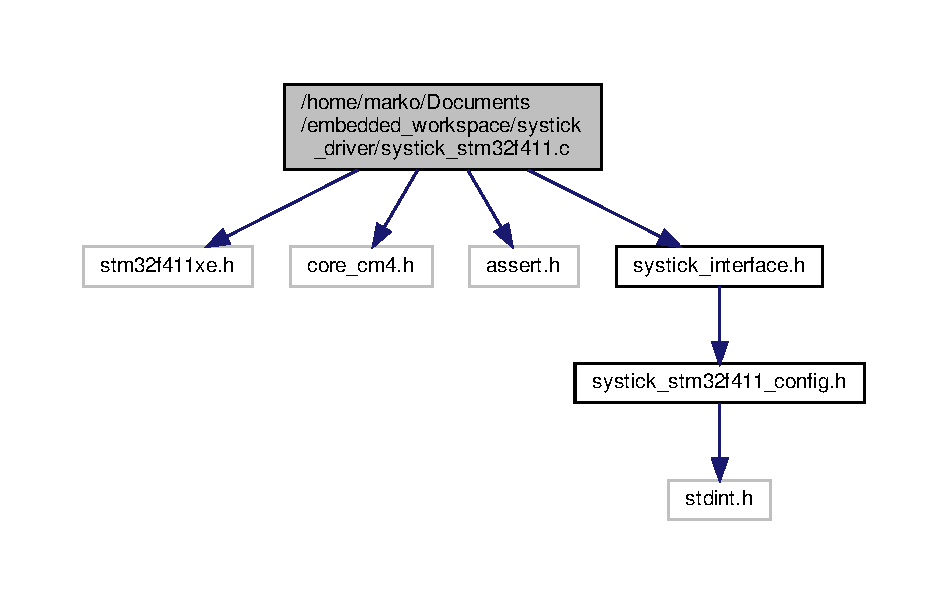
\includegraphics[width=350pt]{systick__stm32f411_8c__incl}
\end{center}
\end{figure}
\subsection*{Macros}
\begin{DoxyCompactItemize}
\item 
\#define \hyperlink{systick__stm32f411_8c_a070d2ce7b6bb7e5c05602aa8c308d0c4}{N\+U\+LL}~(void $\ast$) 0
\end{DoxyCompactItemize}
\subsection*{Functions}
\begin{DoxyCompactItemize}
\item 
void \hyperlink{systick__stm32f411_8c_a05307f714c3701c4b6b396a833f39e92}{systick\+\_\+init} (\hyperlink{structsystick__config__t}{systick\+\_\+config\+\_\+t} $\ast$config)
\item 
void \hyperlink{systick__stm32f411_8c_a6fb10375fe1f7fbef5bdbe3ab33a5376}{systick\+\_\+tick\+\_\+freq\+\_\+set} (\hyperlink{structsystick__config__t}{systick\+\_\+config\+\_\+t} $\ast$config)
\item 
void \hyperlink{systick__stm32f411_8c_ab315ae133959817580ef089539a7ea3f}{systick\+\_\+pause} (void)
\item 
void \hyperlink{systick__stm32f411_8c_abd308166607c7424fb1ae67fb24cba5e}{systick\+\_\+resume} (void)
\item 
void \hyperlink{systick__stm32f411_8c_a618b49039ac69306cc271b98af1fb935}{systick\+\_\+interrupt\+\_\+control} (\hyperlink{systick__stm32f411__config_8h_a82589cfda6cc55b21d80e5e3f47b69d9}{systick\+\_\+interrupt\+\_\+t} interrupt\+\_\+control)
\item 
uint32\+\_\+t \hyperlink{systick__stm32f411_8c_afdf1221fe41470afc9faf278a871b68c}{systick\+\_\+get\+\_\+tick} (void)
\item 
void \hyperlink{systick__stm32f411_8c_ab0275b71c7f7a9080dcac8ffc68559c7}{systick\+\_\+delay} (uint32\+\_\+t delay\+\_\+ms)
\item 
void \hyperlink{systick__stm32f411_8c_a97fc9935ef263cd958116a6ecdfd835f}{systick\+\_\+increment} (void)
\item 
void \hyperlink{systick__stm32f411_8c_a70216cf1d168d9c2239c87878745a631}{systick\+\_\+callback\+\_\+register} (systick\+\_\+callback\+\_\+t callback\+\_\+func)
\item 
void \hyperlink{systick__stm32f411_8c_a8e3818296c4ed279cc0f2967bcdddcee}{systick\+\_\+irq\+\_\+handler} (void)
\end{DoxyCompactItemize}
\subsection*{Variables}
\begin{DoxyCompactItemize}
\item 
static volatile uint32\+\_\+t \hyperlink{systick__stm32f411_8c_ada9acaf0f8242968fb35d628ac9dda27}{tick\+\_\+ms} = 0
\item 
static uint32\+\_\+t \hyperlink{systick__stm32f411_8c_a5973e7102782a9936a5e0d1417863675}{tick\+\_\+freq}
\item 
static systick\+\_\+callback\+\_\+t \hyperlink{systick__stm32f411_8c_a66446d53cda21db96cb43c21d7ddbbf8}{systick\+\_\+callback} = \hyperlink{systick__stm32f411_8c_a97fc9935ef263cd958116a6ecdfd835f}{systick\+\_\+increment}
\end{DoxyCompactItemize}


\subsection{Detailed Description}
Chip specific implementation of systick control. Many functions are pointers to vendor created routines due to the very specific nature of system clocks and ticks. 

\begin{DoxyNote}{Note}
This implementation depends on C\+M\+S\+IS (core\+\_\+cm4.\+h) 
\end{DoxyNote}


\subsection{Macro Definition Documentation}
\mbox{\Hypertarget{systick__stm32f411_8c_a070d2ce7b6bb7e5c05602aa8c308d0c4}\label{systick__stm32f411_8c_a070d2ce7b6bb7e5c05602aa8c308d0c4}} 
\index{systick\+\_\+stm32f411.\+c@{systick\+\_\+stm32f411.\+c}!N\+U\+LL@{N\+U\+LL}}
\index{N\+U\+LL@{N\+U\+LL}!systick\+\_\+stm32f411.\+c@{systick\+\_\+stm32f411.\+c}}
\subsubsection{\texorpdfstring{N\+U\+LL}{NULL}}
{\footnotesize\ttfamily \#define N\+U\+LL~(void $\ast$) 0}

Definition of N\+U\+LL in case it is not defined elsewhere 

\subsection{Function Documentation}
\mbox{\Hypertarget{systick__stm32f411_8c_a70216cf1d168d9c2239c87878745a631}\label{systick__stm32f411_8c_a70216cf1d168d9c2239c87878745a631}} 
\index{systick\+\_\+stm32f411.\+c@{systick\+\_\+stm32f411.\+c}!systick\+\_\+callback\+\_\+register@{systick\+\_\+callback\+\_\+register}}
\index{systick\+\_\+callback\+\_\+register@{systick\+\_\+callback\+\_\+register}!systick\+\_\+stm32f411.\+c@{systick\+\_\+stm32f411.\+c}}
\subsubsection{\texorpdfstring{systick\+\_\+callback\+\_\+register()}{systick\_callback\_register()}}
{\footnotesize\ttfamily void systick\+\_\+callback\+\_\+register (\begin{DoxyParamCaption}\item[{systick\+\_\+callback\+\_\+t}]{callback\+\_\+func }\end{DoxyParamCaption})}

{\bfseries Description\+:} \begin{DoxyVerb}Registers the callback function as the desired on-interrupt functionality.
\end{DoxyVerb}


P\+R\+E-\/\+C\+O\+N\+D\+I\+T\+I\+ON\+: None.

P\+O\+S\+T-\/\+C\+O\+N\+D\+I\+T\+I\+ON\+: the systick\+\_\+callback function pointer variable now points to the desired function


\begin{DoxyParams}{Parameters}
{\em callback\+\_\+func} & a function pointer to a void ($\ast$function)(void) \\
\hline
\end{DoxyParams}
\begin{DoxyReturn}{Returns}
void
\end{DoxyReturn}
{\bfseries Example\+:} 
\begin{DoxyCode}
\hyperlink{systick__interface_8h_a70216cf1d168d9c2239c87878745a631}{systick\_callback\_register}(&interrupt\_behaviour);

\textcolor{comment}{//the irq handler will now call interrupt\_behaviour}
  SysTick\_IRQHandler(\textcolor{keywordtype}{void})
  \{
      \hyperlink{systick__interface_8h_a8e3818296c4ed279cc0f2967bcdddcee}{systick\_irq\_handler}();
  \}
\end{DoxyCode}


\begin{DoxySeeAlso}{See also}
\hyperlink{systick__stm32f411_8c_a8e3818296c4ed279cc0f2967bcdddcee}{systick\+\_\+irq\+\_\+handler}
\end{DoxySeeAlso}
~\newline
{\bfseries  -\/ C\+H\+A\+N\+GE H\+I\+S\+T\+O\+RY -\/ }

\tabulinesep=1mm
\begin{longtabu} spread 0pt [c]{*{4}{|X[-1]}|}
\hline
Date &Software Version &Initials &Description  \\\cline{1-4}
\end{longtabu}
~\newline
~\newline
 

 \mbox{\Hypertarget{systick__stm32f411_8c_ab0275b71c7f7a9080dcac8ffc68559c7}\label{systick__stm32f411_8c_ab0275b71c7f7a9080dcac8ffc68559c7}} 
\index{systick\+\_\+stm32f411.\+c@{systick\+\_\+stm32f411.\+c}!systick\+\_\+delay@{systick\+\_\+delay}}
\index{systick\+\_\+delay@{systick\+\_\+delay}!systick\+\_\+stm32f411.\+c@{systick\+\_\+stm32f411.\+c}}
\subsubsection{\texorpdfstring{systick\+\_\+delay()}{systick\_delay()}}
{\footnotesize\ttfamily void systick\+\_\+delay (\begin{DoxyParamCaption}\item[{uint32\+\_\+t}]{delay\+\_\+ms }\end{DoxyParamCaption})}

{\bfseries Description\+:} \begin{DoxyVerb}Delays the program for the duration of delay_ms in milliseconds
\end{DoxyVerb}


P\+R\+E-\/\+C\+O\+N\+D\+I\+T\+I\+ON\+: None

P\+O\+S\+T-\/\+C\+O\+N\+D\+I\+T\+I\+ON\+: delay\+\_\+ms have gone by and the rest of the program will resume


\begin{DoxyParams}{Parameters}
{\em delay\+\_\+ms} & is the length of time the user wishes to way\\
\hline
\end{DoxyParams}
\begin{DoxyReturn}{Returns}
void
\end{DoxyReturn}
{\bfseries Example\+:} 


\begin{DoxyCode}
\hyperlink{systick__interface_8h_ab0275b71c7f7a9080dcac8ffc68559c7}{systick\_delay}(200);
\end{DoxyCode}


\begin{DoxySeeAlso}{See also}
\hyperlink{systick__stm32f411_8c_a6fb10375fe1f7fbef5bdbe3ab33a5376}{systick\+\_\+tick\+\_\+freq\+\_\+set} 

\hyperlink{systick__stm32f411_8c_afdf1221fe41470afc9faf278a871b68c}{systick\+\_\+get\+\_\+tick}
\end{DoxySeeAlso}
~\newline
{\bfseries  -\/ C\+H\+A\+N\+GE H\+I\+S\+T\+O\+RY -\/ }

\tabulinesep=1mm
\begin{longtabu} spread 0pt [c]{*{4}{|X[-1]}|}
\hline
Date &Software Version &Initials &Description  \\\cline{1-4}
\end{longtabu}
~\newline
~\newline
 

 \mbox{\Hypertarget{systick__stm32f411_8c_afdf1221fe41470afc9faf278a871b68c}\label{systick__stm32f411_8c_afdf1221fe41470afc9faf278a871b68c}} 
\index{systick\+\_\+stm32f411.\+c@{systick\+\_\+stm32f411.\+c}!systick\+\_\+get\+\_\+tick@{systick\+\_\+get\+\_\+tick}}
\index{systick\+\_\+get\+\_\+tick@{systick\+\_\+get\+\_\+tick}!systick\+\_\+stm32f411.\+c@{systick\+\_\+stm32f411.\+c}}
\subsubsection{\texorpdfstring{systick\+\_\+get\+\_\+tick()}{systick\_get\_tick()}}
{\footnotesize\ttfamily uint32\+\_\+t systick\+\_\+get\+\_\+tick (\begin{DoxyParamCaption}\item[{void}]{ }\end{DoxyParamCaption})}

{\bfseries Description\+:} \begin{DoxyVerb}DReturns the current value of the tick_ms variable
\end{DoxyVerb}


P\+R\+E-\/\+C\+O\+N\+D\+I\+T\+I\+ON\+: None

P\+O\+S\+T-\/\+C\+O\+N\+D\+I\+T\+I\+ON\+: The function has returned the current value of the tick variable.

\begin{DoxyReturn}{Returns}
uint32\+\_\+t the current tick value
\end{DoxyReturn}
{\bfseries Example\+:} 


\begin{DoxyCode}
uint32\_t current\_tick = \hyperlink{systick__interface_8h_afdf1221fe41470afc9faf278a871b68c}{systick\_get\_tick}();
\end{DoxyCode}


\begin{DoxySeeAlso}{See also}
\hyperlink{systick__stm32f411_8c_a6fb10375fe1f7fbef5bdbe3ab33a5376}{systick\+\_\+tick\+\_\+freq\+\_\+set} 

\hyperlink{systick__stm32f411_8c_ab0275b71c7f7a9080dcac8ffc68559c7}{systick\+\_\+delay}
\end{DoxySeeAlso}
~\newline
{\bfseries  -\/ C\+H\+A\+N\+GE H\+I\+S\+T\+O\+RY -\/ }

\tabulinesep=1mm
\begin{longtabu} spread 0pt [c]{*{4}{|X[-1]}|}
\hline
Date &Software Version &Initials &Description  \\\cline{1-4}
\end{longtabu}
~\newline
~\newline
 

 \mbox{\Hypertarget{systick__stm32f411_8c_a97fc9935ef263cd958116a6ecdfd835f}\label{systick__stm32f411_8c_a97fc9935ef263cd958116a6ecdfd835f}} 
\index{systick\+\_\+stm32f411.\+c@{systick\+\_\+stm32f411.\+c}!systick\+\_\+increment@{systick\+\_\+increment}}
\index{systick\+\_\+increment@{systick\+\_\+increment}!systick\+\_\+stm32f411.\+c@{systick\+\_\+stm32f411.\+c}}
\subsubsection{\texorpdfstring{systick\+\_\+increment()}{systick\_increment()}}
{\footnotesize\ttfamily void systick\+\_\+increment (\begin{DoxyParamCaption}\item[{void}]{ }\end{DoxyParamCaption})}

{\bfseries Description\+:} \begin{DoxyVerb}Increments the tick by the number of milliseconds between systick register
overflows. Called within systick_irq_handler.
\end{DoxyVerb}


P\+R\+E-\/\+C\+O\+N\+D\+I\+T\+I\+ON\+: None.

P\+O\+S\+T-\/\+C\+O\+N\+D\+I\+T\+I\+ON\+: tick\+\_\+ms has incremented by tick\+\_\+freq milliseconds

\begin{DoxyReturn}{Returns}
void
\end{DoxyReturn}
{\bfseries Example\+:} 
\begin{DoxyCode}
\textcolor{comment}{//By default is called automatically upon SysTick interrupt}
  SysTick\_IRQHandler(\textcolor{keywordtype}{void})
  \{
      \hyperlink{systick__interface_8h_a8e3818296c4ed279cc0f2967bcdddcee}{systick\_irq\_handler}();
  \}
\end{DoxyCode}


\begin{DoxySeeAlso}{See also}
\hyperlink{systick__stm32f411_8c_a70216cf1d168d9c2239c87878745a631}{systick\+\_\+callback\+\_\+register} 

\hyperlink{systick__stm32f411_8c_a8e3818296c4ed279cc0f2967bcdddcee}{systick\+\_\+irq\+\_\+handler}
\end{DoxySeeAlso}
~\newline
{\bfseries  -\/ C\+H\+A\+N\+GE H\+I\+S\+T\+O\+RY -\/ }

\tabulinesep=1mm
\begin{longtabu} spread 0pt [c]{*{4}{|X[-1]}|}
\hline
Date &Software Version &Initials &Description  \\\cline{1-4}
\end{longtabu}
~\newline
~\newline
 

 \mbox{\Hypertarget{systick__stm32f411_8c_a05307f714c3701c4b6b396a833f39e92}\label{systick__stm32f411_8c_a05307f714c3701c4b6b396a833f39e92}} 
\index{systick\+\_\+stm32f411.\+c@{systick\+\_\+stm32f411.\+c}!systick\+\_\+init@{systick\+\_\+init}}
\index{systick\+\_\+init@{systick\+\_\+init}!systick\+\_\+stm32f411.\+c@{systick\+\_\+stm32f411.\+c}}
\subsubsection{\texorpdfstring{systick\+\_\+init()}{systick\_init()}}
{\footnotesize\ttfamily void systick\+\_\+init (\begin{DoxyParamCaption}\item[{\hyperlink{structsystick__config__t}{systick\+\_\+config\+\_\+t} $\ast$}]{config }\end{DoxyParamCaption})}

{\bfseries Description\+:} \begin{DoxyVerb}Carries out the initialisation of the the systick based on information in the
config table
\end{DoxyVerb}


P\+R\+E-\/\+C\+O\+N\+D\+I\+T\+I\+ON\+: The clock system (R\+CC) has been initialised. P\+R\+E-\/\+C\+O\+N\+D\+I\+T\+I\+ON\+: The desired frequency (tick\+\_\+freq\+\_\+khz) results in a number small enough to fit the 0x\+F\+F\+F\+F\+FF mask P\+R\+E-\/\+C\+O\+N\+D\+I\+T\+I\+ON\+: (Soft Assert) the systick is enabled through its config register

P\+O\+S\+T-\/\+C\+O\+N\+D\+I\+T\+I\+ON\+: The systick has been configured to count with the desired frequency P\+O\+S\+T-\/\+C\+O\+N\+D\+I\+T\+I\+ON\+: The systick interrupt has been enabled (if desired) and its priority set to maximum. P\+O\+S\+T-\/\+C\+O\+N\+D\+I\+T\+I\+ON\+: The systick clock source has been set to the desired option


\begin{DoxyParams}{Parameters}
{\em config} & a pointer to the systick configuration structure\\
\hline
\end{DoxyParams}
\begin{DoxyReturn}{Returns}
void
\end{DoxyReturn}
{\bfseries Example\+:} 


\begin{DoxyCode}
\hyperlink{structsystick__config__t}{systick\_config\_t} *tick\_config = \hyperlink{systick__stm32f411__config_8c_a736aba702662d732de33f92b1fef7ad0}{systick\_config\_get}();
\hyperlink{systick__interface_8h_a05307f714c3701c4b6b396a833f39e92}{systick\_init}(tick\_config);
\end{DoxyCode}


\begin{DoxySeeAlso}{See also}
\hyperlink{systick__stm32f411__config_8h_a736aba702662d732de33f92b1fef7ad0}{systick\+\_\+config\+\_\+get} 

\hyperlink{systick__stm32f411_8c_a6fb10375fe1f7fbef5bdbe3ab33a5376}{systick\+\_\+tick\+\_\+freq\+\_\+set} 

\hyperlink{systick__stm32f411_8c_ab315ae133959817580ef089539a7ea3f}{systick\+\_\+pause} 

\hyperlink{systick__stm32f411_8c_abd308166607c7424fb1ae67fb24cba5e}{systick\+\_\+resume} 

\hyperlink{systick__stm32f411_8c_a618b49039ac69306cc271b98af1fb935}{systick\+\_\+interrupt\+\_\+control} ~\newline
{\bfseries  -\/ C\+H\+A\+N\+GE H\+I\+S\+T\+O\+RY -\/ }
\end{DoxySeeAlso}
\tabulinesep=1mm
\begin{longtabu} spread 0pt [c]{*{4}{|X[-1]}|}
\hline
Date &Software Version &Initials &Description  \\\cline{1-4}
\end{longtabu}
~\newline
~\newline
 

 \mbox{\Hypertarget{systick__stm32f411_8c_a618b49039ac69306cc271b98af1fb935}\label{systick__stm32f411_8c_a618b49039ac69306cc271b98af1fb935}} 
\index{systick\+\_\+stm32f411.\+c@{systick\+\_\+stm32f411.\+c}!systick\+\_\+interrupt\+\_\+control@{systick\+\_\+interrupt\+\_\+control}}
\index{systick\+\_\+interrupt\+\_\+control@{systick\+\_\+interrupt\+\_\+control}!systick\+\_\+stm32f411.\+c@{systick\+\_\+stm32f411.\+c}}
\subsubsection{\texorpdfstring{systick\+\_\+interrupt\+\_\+control()}{systick\_interrupt\_control()}}
{\footnotesize\ttfamily void systick\+\_\+interrupt\+\_\+control (\begin{DoxyParamCaption}\item[{\hyperlink{systick__stm32f411__config_8h_a82589cfda6cc55b21d80e5e3f47b69d9}{systick\+\_\+interrupt\+\_\+t}}]{interrupt\+\_\+control }\end{DoxyParamCaption})}

{\bfseries Description\+:} \begin{DoxyVerb}Enables or disables the systick interrupt
\end{DoxyVerb}


P\+R\+E-\/\+C\+O\+N\+D\+I\+T\+I\+ON\+: (Soft Assert) The systick is paused

P\+O\+S\+T-\/\+C\+O\+N\+D\+I\+T\+I\+ON\+: The systick interrupt is enabled or disabled, as per the input


\begin{DoxyParams}{Parameters}
{\em systick\+\_\+interrupt\+\_\+t} & Control parameter defining if the interrupt will be activated or deactivated \\
\hline
\end{DoxyParams}
\begin{DoxyReturn}{Returns}
void
\end{DoxyReturn}
{\bfseries Example\+:} 


\begin{DoxyCode}
\hyperlink{systick__interface_8h_ab315ae133959817580ef089539a7ea3f}{systick\_pause}();
\hyperlink{systick__interface_8h_a618b49039ac69306cc271b98af1fb935}{systick\_interrupt\_control}(SYSTICK\_INT\_ENABLED);
\hyperlink{systick__interface_8h_abd308166607c7424fb1ae67fb24cba5e}{systick\_resume}();
\end{DoxyCode}


\begin{DoxySeeAlso}{See also}
\hyperlink{systick__stm32f411_8c_a05307f714c3701c4b6b396a833f39e92}{systick\+\_\+init} 

\hyperlink{systick__stm32f411_8c_a6fb10375fe1f7fbef5bdbe3ab33a5376}{systick\+\_\+tick\+\_\+freq\+\_\+set} 

\hyperlink{systick__stm32f411_8c_ab315ae133959817580ef089539a7ea3f}{systick\+\_\+pause} 

\hyperlink{systick__stm32f411_8c_abd308166607c7424fb1ae67fb24cba5e}{systick\+\_\+resume}
\end{DoxySeeAlso}
~\newline
{\bfseries  -\/ C\+H\+A\+N\+GE H\+I\+S\+T\+O\+RY -\/ }

\tabulinesep=1mm
\begin{longtabu} spread 0pt [c]{*{4}{|X[-1]}|}
\hline
Date &Software Version &Initials &Description  \\\cline{1-4}
\end{longtabu}
~\newline
~\newline
 

 \mbox{\Hypertarget{systick__stm32f411_8c_a8e3818296c4ed279cc0f2967bcdddcee}\label{systick__stm32f411_8c_a8e3818296c4ed279cc0f2967bcdddcee}} 
\index{systick\+\_\+stm32f411.\+c@{systick\+\_\+stm32f411.\+c}!systick\+\_\+irq\+\_\+handler@{systick\+\_\+irq\+\_\+handler}}
\index{systick\+\_\+irq\+\_\+handler@{systick\+\_\+irq\+\_\+handler}!systick\+\_\+stm32f411.\+c@{systick\+\_\+stm32f411.\+c}}
\subsubsection{\texorpdfstring{systick\+\_\+irq\+\_\+handler()}{systick\_irq\_handler()}}
{\footnotesize\ttfamily void systick\+\_\+irq\+\_\+handler (\begin{DoxyParamCaption}\item[{void}]{ }\end{DoxyParamCaption})}

{\bfseries Description\+:} \begin{DoxyVerb}Calls the systick callback function. The default callback is systick_increment.
\end{DoxyVerb}


P\+R\+E-\/\+C\+O\+N\+D\+I\+T\+I\+ON\+: The callback function is non-\/\+N\+U\+LL

P\+O\+S\+T-\/\+C\+O\+N\+D\+I\+T\+I\+ON\+: the systick\+\_\+callback function is called

\begin{DoxyReturn}{Returns}
void
\end{DoxyReturn}
{\bfseries Example\+:} 
\begin{DoxyCode}
\hyperlink{systick__interface_8h_a70216cf1d168d9c2239c87878745a631}{systick\_callback\_register}(&interrupt\_behaviour);

\textcolor{comment}{//the irq handler will now call interrupt\_behaviour}
  SysTick\_IRQHandler(\textcolor{keywordtype}{void})
  \{
      \hyperlink{systick__interface_8h_a8e3818296c4ed279cc0f2967bcdddcee}{systick\_irq\_handler}();
  \}
\end{DoxyCode}


\begin{DoxySeeAlso}{See also}
\hyperlink{systick__stm32f411_8c_a70216cf1d168d9c2239c87878745a631}{systick\+\_\+callback\+\_\+register} 

\hyperlink{systick__stm32f411_8c_a97fc9935ef263cd958116a6ecdfd835f}{systick\+\_\+increment}
\end{DoxySeeAlso}
~\newline
{\bfseries  -\/ C\+H\+A\+N\+GE H\+I\+S\+T\+O\+RY -\/ }

\tabulinesep=1mm
\begin{longtabu} spread 0pt [c]{*{4}{|X[-1]}|}
\hline
Date &Software Version &Initials &Description  \\\cline{1-4}
\end{longtabu}
~\newline
~\newline
 

 \mbox{\Hypertarget{systick__stm32f411_8c_ab315ae133959817580ef089539a7ea3f}\label{systick__stm32f411_8c_ab315ae133959817580ef089539a7ea3f}} 
\index{systick\+\_\+stm32f411.\+c@{systick\+\_\+stm32f411.\+c}!systick\+\_\+pause@{systick\+\_\+pause}}
\index{systick\+\_\+pause@{systick\+\_\+pause}!systick\+\_\+stm32f411.\+c@{systick\+\_\+stm32f411.\+c}}
\subsubsection{\texorpdfstring{systick\+\_\+pause()}{systick\_pause()}}
{\footnotesize\ttfamily void systick\+\_\+pause (\begin{DoxyParamCaption}\item[{void}]{ }\end{DoxyParamCaption})}

{\bfseries Description\+:} \begin{DoxyVerb}Pauses the counting of the systick.
\end{DoxyVerb}


P\+R\+E-\/\+C\+O\+N\+D\+I\+T\+I\+ON\+: None

P\+O\+S\+T-\/\+C\+O\+N\+D\+I\+T\+I\+ON\+: The systick timer is paused

\begin{DoxyReturn}{Returns}
void
\end{DoxyReturn}
{\bfseries Example\+:} 


\begin{DoxyCode}
\hyperlink{systick__interface_8h_ab315ae133959817580ef089539a7ea3f}{systick\_pause}();
\textcolor{comment}{//... do things....}
\hyperlink{systick__interface_8h_abd308166607c7424fb1ae67fb24cba5e}{systick\_resume}();
\end{DoxyCode}


\begin{DoxySeeAlso}{See also}
\hyperlink{systick__stm32f411_8c_a6fb10375fe1f7fbef5bdbe3ab33a5376}{systick\+\_\+tick\+\_\+freq\+\_\+set} 

\hyperlink{systick__stm32f411_8c_abd308166607c7424fb1ae67fb24cba5e}{systick\+\_\+resume}
\end{DoxySeeAlso}
~\newline
{\bfseries  -\/ C\+H\+A\+N\+GE H\+I\+S\+T\+O\+RY -\/ }

\tabulinesep=1mm
\begin{longtabu} spread 0pt [c]{*{4}{|X[-1]}|}
\hline
Date &Software Version &Initials &Description  \\\cline{1-4}
\end{longtabu}
~\newline
~\newline
 

 \mbox{\Hypertarget{systick__stm32f411_8c_abd308166607c7424fb1ae67fb24cba5e}\label{systick__stm32f411_8c_abd308166607c7424fb1ae67fb24cba5e}} 
\index{systick\+\_\+stm32f411.\+c@{systick\+\_\+stm32f411.\+c}!systick\+\_\+resume@{systick\+\_\+resume}}
\index{systick\+\_\+resume@{systick\+\_\+resume}!systick\+\_\+stm32f411.\+c@{systick\+\_\+stm32f411.\+c}}
\subsubsection{\texorpdfstring{systick\+\_\+resume()}{systick\_resume()}}
{\footnotesize\ttfamily void systick\+\_\+resume (\begin{DoxyParamCaption}\item[{void}]{ }\end{DoxyParamCaption})}

{\bfseries Description\+:} \begin{DoxyVerb}Resume the counting of the systick.
\end{DoxyVerb}


P\+R\+E-\/\+C\+O\+N\+D\+I\+T\+I\+ON\+: None

P\+O\+S\+T-\/\+C\+O\+N\+D\+I\+T\+I\+ON\+: The systick timer is running

\begin{DoxyReturn}{Returns}
void
\end{DoxyReturn}
{\bfseries Example\+:} 


\begin{DoxyCode}
\hyperlink{systick__interface_8h_ab315ae133959817580ef089539a7ea3f}{systick\_pause}();
\textcolor{comment}{//... do things....}
\hyperlink{systick__interface_8h_abd308166607c7424fb1ae67fb24cba5e}{systick\_resume}();
\end{DoxyCode}


\begin{DoxySeeAlso}{See also}
\hyperlink{systick__stm32f411_8c_a6fb10375fe1f7fbef5bdbe3ab33a5376}{systick\+\_\+tick\+\_\+freq\+\_\+set} 

\hyperlink{systick__stm32f411_8c_ab315ae133959817580ef089539a7ea3f}{systick\+\_\+pause}
\end{DoxySeeAlso}
~\newline
{\bfseries  -\/ C\+H\+A\+N\+GE H\+I\+S\+T\+O\+RY -\/ }

\tabulinesep=1mm
\begin{longtabu} spread 0pt [c]{*{4}{|X[-1]}|}
\hline
Date &Software Version &Initials &Description  \\\cline{1-4}
\end{longtabu}
~\newline
~\newline
 

 \mbox{\Hypertarget{systick__stm32f411_8c_a6fb10375fe1f7fbef5bdbe3ab33a5376}\label{systick__stm32f411_8c_a6fb10375fe1f7fbef5bdbe3ab33a5376}} 
\index{systick\+\_\+stm32f411.\+c@{systick\+\_\+stm32f411.\+c}!systick\+\_\+tick\+\_\+freq\+\_\+set@{systick\+\_\+tick\+\_\+freq\+\_\+set}}
\index{systick\+\_\+tick\+\_\+freq\+\_\+set@{systick\+\_\+tick\+\_\+freq\+\_\+set}!systick\+\_\+stm32f411.\+c@{systick\+\_\+stm32f411.\+c}}
\subsubsection{\texorpdfstring{systick\+\_\+tick\+\_\+freq\+\_\+set()}{systick\_tick\_freq\_set()}}
{\footnotesize\ttfamily void systick\+\_\+tick\+\_\+freq\+\_\+set (\begin{DoxyParamCaption}\item[{\hyperlink{structsystick__config__t}{systick\+\_\+config\+\_\+t} $\ast$}]{config }\end{DoxyParamCaption})}

{\bfseries Description\+:} \begin{DoxyVerb}Sets the frequency of the systick update to the desired value in kHz.
\end{DoxyVerb}


P\+R\+E-\/\+C\+O\+N\+D\+I\+T\+I\+ON\+: The desired frequency (tick\+\_\+freq\+\_\+khz) results in a number small enough to fit the 0x\+F\+F\+F\+F\+FF mask P\+R\+E-\/\+C\+O\+N\+D\+I\+T\+I\+ON\+: (Soft Assert) the systick is enabled through its config register P\+R\+E-\/\+C\+O\+N\+D\+I\+T\+I\+ON\+: (Soft Assert) the systick is paused

P\+O\+S\+T-\/\+C\+O\+N\+D\+I\+T\+I\+ON\+: The systick has been configured to count with the desired frequency


\begin{DoxyParams}{Parameters}
{\em config} & a pointer to the systick configuration structure\\
\hline
\end{DoxyParams}
\begin{DoxyReturn}{Returns}
void
\end{DoxyReturn}
{\bfseries Example\+:} 


\begin{DoxyCode}
\hyperlink{structsystick__config__t}{systick\_config\_t} *tick\_config = \hyperlink{systick__stm32f411__config_8c_a736aba702662d732de33f92b1fef7ad0}{systick\_config\_get}();
\hyperlink{systick__interface_8h_a05307f714c3701c4b6b396a833f39e92}{systick\_init}(tick\_config);
\textcolor{comment}{//... later ...}
\hyperlink{systick__interface_8h_ab315ae133959817580ef089539a7ea3f}{systick\_pause}();
tick\_config->\hyperlink{structsystick__config__t_a5d1767c41ce5e869439e7197fd6a7373}{tick\_freq\_khz} = 5; \textcolor{comment}{//kHz}
\hyperlink{systick__interface_8h_a6fb10375fe1f7fbef5bdbe3ab33a5376}{systick\_tick\_freq\_set}(tick\_config);
\hyperlink{systick__interface_8h_abd308166607c7424fb1ae67fb24cba5e}{systick\_resume}();
\end{DoxyCode}


\begin{DoxySeeAlso}{See also}
\hyperlink{systick__stm32f411_8c_a05307f714c3701c4b6b396a833f39e92}{systick\+\_\+init} 

\hyperlink{systick__stm32f411__config_8h_a736aba702662d732de33f92b1fef7ad0}{systick\+\_\+config\+\_\+get} 

\hyperlink{systick__stm32f411_8c_ab315ae133959817580ef089539a7ea3f}{systick\+\_\+pause} 

\hyperlink{systick__stm32f411_8c_abd308166607c7424fb1ae67fb24cba5e}{systick\+\_\+resume} ~\newline
{\bfseries  -\/ C\+H\+A\+N\+GE H\+I\+S\+T\+O\+RY -\/ }
\end{DoxySeeAlso}
\tabulinesep=1mm
\begin{longtabu} spread 0pt [c]{*{4}{|X[-1]}|}
\hline
Date &Software Version &Initials &Description  \\\cline{1-4}
\end{longtabu}
~\newline
~\newline
 

 

\subsection{Variable Documentation}
\mbox{\Hypertarget{systick__stm32f411_8c_a66446d53cda21db96cb43c21d7ddbbf8}\label{systick__stm32f411_8c_a66446d53cda21db96cb43c21d7ddbbf8}} 
\index{systick\+\_\+stm32f411.\+c@{systick\+\_\+stm32f411.\+c}!systick\+\_\+callback@{systick\+\_\+callback}}
\index{systick\+\_\+callback@{systick\+\_\+callback}!systick\+\_\+stm32f411.\+c@{systick\+\_\+stm32f411.\+c}}
\subsubsection{\texorpdfstring{systick\+\_\+callback}{systick\_callback}}
{\footnotesize\ttfamily systick\+\_\+callback\+\_\+t systick\+\_\+callback = \hyperlink{systick__stm32f411_8c_a97fc9935ef263cd958116a6ecdfd835f}{systick\+\_\+increment}\hspace{0.3cm}{\ttfamily [static]}}

Callback function which will be dereferenced upon systick interrupts Default value is systick\+\_\+increment, but can be changed through the callback\+\_\+register function \mbox{\Hypertarget{systick__stm32f411_8c_a5973e7102782a9936a5e0d1417863675}\label{systick__stm32f411_8c_a5973e7102782a9936a5e0d1417863675}} 
\index{systick\+\_\+stm32f411.\+c@{systick\+\_\+stm32f411.\+c}!tick\+\_\+freq@{tick\+\_\+freq}}
\index{tick\+\_\+freq@{tick\+\_\+freq}!systick\+\_\+stm32f411.\+c@{systick\+\_\+stm32f411.\+c}}
\subsubsection{\texorpdfstring{tick\+\_\+freq}{tick\_freq}}
{\footnotesize\ttfamily uint32\+\_\+t tick\+\_\+freq\hspace{0.3cm}{\ttfamily [static]}}

Tick frequency (increment rate) \mbox{\Hypertarget{systick__stm32f411_8c_ada9acaf0f8242968fb35d628ac9dda27}\label{systick__stm32f411_8c_ada9acaf0f8242968fb35d628ac9dda27}} 
\index{systick\+\_\+stm32f411.\+c@{systick\+\_\+stm32f411.\+c}!tick\+\_\+ms@{tick\+\_\+ms}}
\index{tick\+\_\+ms@{tick\+\_\+ms}!systick\+\_\+stm32f411.\+c@{systick\+\_\+stm32f411.\+c}}
\subsubsection{\texorpdfstring{tick\+\_\+ms}{tick\_ms}}
{\footnotesize\ttfamily volatile uint32\+\_\+t tick\+\_\+ms = 0\hspace{0.3cm}{\ttfamily [static]}}

Encapsulated tick value 
\hypertarget{systick__stm32f411__config_8c}{}\section{/home/marko/\+Documents/embedded\+\_\+workspace/systick\+\_\+driver/systick\+\_\+stm32f411\+\_\+config.c File Reference}
\label{systick__stm32f411__config_8c}\index{/home/marko/\+Documents/embedded\+\_\+workspace/systick\+\_\+driver/systick\+\_\+stm32f411\+\_\+config.\+c@{/home/marko/\+Documents/embedded\+\_\+workspace/systick\+\_\+driver/systick\+\_\+stm32f411\+\_\+config.\+c}}


Contains the configuration information for the systick.  


{\ttfamily \#include \char`\"{}systick\+\_\+stm32f411\+\_\+config.\+h\char`\"{}}\newline
Include dependency graph for systick\+\_\+stm32f411\+\_\+config.\+c\+:
\nopagebreak
\begin{figure}[H]
\begin{center}
\leavevmode
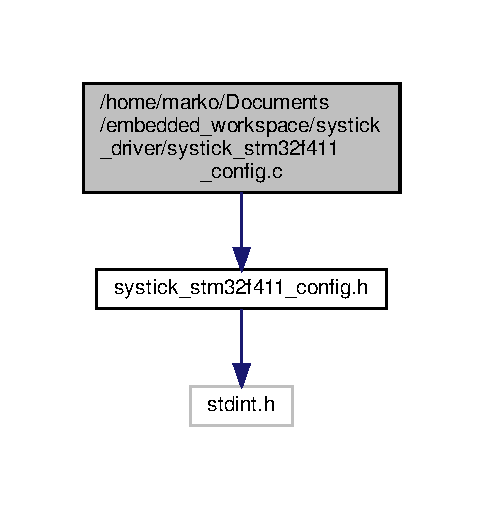
\includegraphics[width=232pt]{systick__stm32f411__config_8c__incl}
\end{center}
\end{figure}
\subsection*{Functions}
\begin{DoxyCompactItemize}
\item 
const \hyperlink{structsystick__config__t}{systick\+\_\+config\+\_\+t} $\ast$ \hyperlink{systick__stm32f411__config_8c_a736aba702662d732de33f92b1fef7ad0}{systick\+\_\+config\+\_\+get} (void)
\end{DoxyCompactItemize}
\subsection*{Variables}
\begin{DoxyCompactItemize}
\item 
static const \hyperlink{structsystick__config__t}{systick\+\_\+config\+\_\+t} \hyperlink{systick__stm32f411__config_8c_a9a1607434b9bc6fc26d7796141f02069}{systick\+\_\+config\+\_\+table} \mbox{[}N\+U\+M\+\_\+\+S\+Y\+S\+T\+I\+C\+KS\mbox{]}
\end{DoxyCompactItemize}


\subsection{Detailed Description}
Contains the configuration information for the systick. 



\subsection{Function Documentation}
\mbox{\Hypertarget{systick__stm32f411__config_8c_a736aba702662d732de33f92b1fef7ad0}\label{systick__stm32f411__config_8c_a736aba702662d732de33f92b1fef7ad0}} 
\index{systick\+\_\+stm32f411\+\_\+config.\+c@{systick\+\_\+stm32f411\+\_\+config.\+c}!systick\+\_\+config\+\_\+get@{systick\+\_\+config\+\_\+get}}
\index{systick\+\_\+config\+\_\+get@{systick\+\_\+config\+\_\+get}!systick\+\_\+stm32f411\+\_\+config.\+c@{systick\+\_\+stm32f411\+\_\+config.\+c}}
\subsubsection{\texorpdfstring{systick\+\_\+config\+\_\+get()}{systick\_config\_get()}}
{\footnotesize\ttfamily const \hyperlink{structsystick__config__t}{systick\+\_\+config\+\_\+t}$\ast$ systick\+\_\+config\+\_\+get (\begin{DoxyParamCaption}\item[{void}]{ }\end{DoxyParamCaption})}

Function returning a pointer to the (quite protected) config data 

\subsection{Variable Documentation}
\mbox{\Hypertarget{systick__stm32f411__config_8c_a9a1607434b9bc6fc26d7796141f02069}\label{systick__stm32f411__config_8c_a9a1607434b9bc6fc26d7796141f02069}} 
\index{systick\+\_\+stm32f411\+\_\+config.\+c@{systick\+\_\+stm32f411\+\_\+config.\+c}!systick\+\_\+config\+\_\+table@{systick\+\_\+config\+\_\+table}}
\index{systick\+\_\+config\+\_\+table@{systick\+\_\+config\+\_\+table}!systick\+\_\+stm32f411\+\_\+config.\+c@{systick\+\_\+stm32f411\+\_\+config.\+c}}
\subsubsection{\texorpdfstring{systick\+\_\+config\+\_\+table}{systick\_config\_table}}
{\footnotesize\ttfamily const \hyperlink{structsystick__config__t}{systick\+\_\+config\+\_\+t} systick\+\_\+config\+\_\+table\mbox{[}N\+U\+M\+\_\+\+S\+Y\+S\+T\+I\+C\+KS\mbox{]}\hspace{0.3cm}{\ttfamily [static]}}

{\bfseries Initial value\+:}
\begin{DoxyCode}
=
\{   
                                            
        \{SYSTICK\_ENABLED,    1,         SYSTICK\_INT\_ENABLED,    SYSTICK\_INTERNAL\_CLOCK\}
\}
\end{DoxyCode}
Table containing config information for the configuration of the systick. Populated at first with default values 
\hypertarget{systick__stm32f411__config_8h}{}\section{/home/marko/\+Documents/embedded\+\_\+workspace/systick\+\_\+driver/systick\+\_\+stm32f411\+\_\+config.h File Reference}
\label{systick__stm32f411__config_8h}\index{/home/marko/\+Documents/embedded\+\_\+workspace/systick\+\_\+driver/systick\+\_\+stm32f411\+\_\+config.\+h@{/home/marko/\+Documents/embedded\+\_\+workspace/systick\+\_\+driver/systick\+\_\+stm32f411\+\_\+config.\+h}}


Chip specific header containing all relevant enums and structs to configure the systick.  


{\ttfamily \#include $<$stdint.\+h$>$}\newline
Include dependency graph for systick\+\_\+stm32f411\+\_\+config.\+h\+:
\nopagebreak
\begin{figure}[H]
\begin{center}
\leavevmode
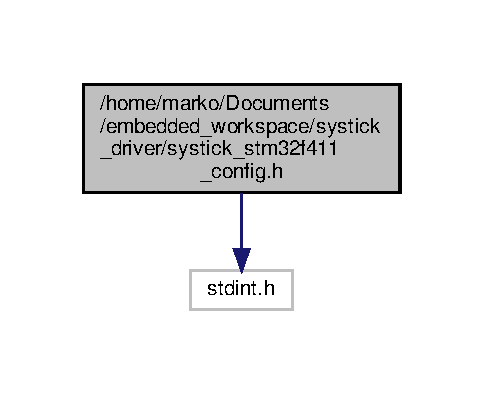
\includegraphics[width=232pt]{systick__stm32f411__config_8h__incl}
\end{center}
\end{figure}
This graph shows which files directly or indirectly include this file\+:
\nopagebreak
\begin{figure}[H]
\begin{center}
\leavevmode
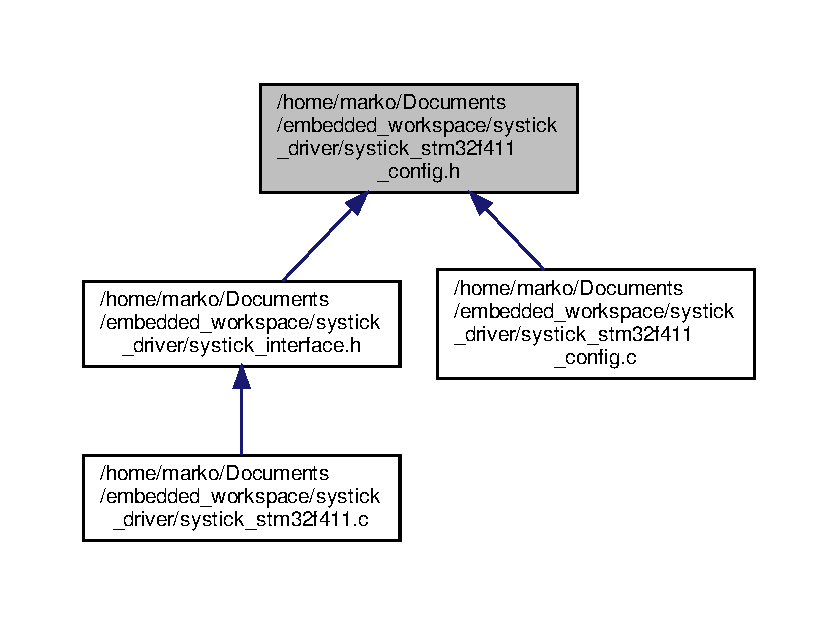
\includegraphics[width=350pt]{systick__stm32f411__config_8h__dep__incl}
\end{center}
\end{figure}
\subsection*{Data Structures}
\begin{DoxyCompactItemize}
\item 
struct \hyperlink{structsystick__config__t}{systick\+\_\+config\+\_\+t}
\end{DoxyCompactItemize}
\subsection*{Enumerations}
\begin{DoxyCompactItemize}
\item 
\mbox{\Hypertarget{systick__stm32f411__config_8h_a13339cd298c9dda78016a52890c456f4}\label{systick__stm32f411__config_8h_a13339cd298c9dda78016a52890c456f4}} 
enum {\bfseries systick\+\_\+t} \{ {\bfseries S\+Y\+S\+T\+I\+C\+K\+\_\+1}, 
{\bfseries N\+U\+M\+\_\+\+S\+Y\+S\+T\+I\+C\+KS}
 \}
\item 
enum \hyperlink{systick__stm32f411__config_8h_a54abff3d12292257e357d04094ebc415}{systick\+\_\+enabled\+\_\+t} \{ {\bfseries S\+Y\+S\+T\+I\+C\+K\+\_\+\+D\+I\+S\+A\+B\+L\+ED}, 
{\bfseries S\+Y\+S\+T\+I\+C\+K\+\_\+\+E\+N\+A\+B\+L\+ED}
 \}
\item 
enum \hyperlink{systick__stm32f411__config_8h_a82589cfda6cc55b21d80e5e3f47b69d9}{systick\+\_\+interrupt\+\_\+t} \{ {\bfseries S\+Y\+S\+T\+I\+C\+K\+\_\+\+I\+N\+T\+\_\+\+D\+I\+S\+A\+B\+L\+ED}, 
{\bfseries S\+Y\+S\+T\+I\+C\+K\+\_\+\+I\+N\+T\+\_\+\+E\+N\+A\+B\+L\+ED}
 \}
\item 
enum \hyperlink{systick__stm32f411__config_8h_a39469603d3120252cd4f82defbd9525e}{systick\+\_\+clock\+\_\+source\+\_\+t} \{ {\bfseries S\+Y\+S\+T\+I\+C\+K\+\_\+\+E\+X\+T\+E\+R\+N\+A\+L\+\_\+\+C\+L\+O\+CK}, 
{\bfseries S\+Y\+S\+T\+I\+C\+K\+\_\+\+I\+N\+T\+E\+R\+N\+A\+L\+\_\+\+C\+L\+O\+CK}
 \}
\end{DoxyCompactItemize}
\subsection*{Functions}
\begin{DoxyCompactItemize}
\item 
const \hyperlink{structsystick__config__t}{systick\+\_\+config\+\_\+t} $\ast$ \hyperlink{systick__stm32f411__config_8h_a736aba702662d732de33f92b1fef7ad0}{systick\+\_\+config\+\_\+get} (void)
\end{DoxyCompactItemize}
\subsection*{Variables}
\begin{DoxyCompactItemize}
\item 
uint32\+\_\+t \hyperlink{systick__stm32f411__config_8h_aa3cd3e43291e81e795d642b79b6088e6}{System\+Core\+Clock}
\end{DoxyCompactItemize}


\subsection{Detailed Description}
Chip specific header containing all relevant enums and structs to configure the systick. 



\subsection{Enumeration Type Documentation}
\mbox{\Hypertarget{systick__stm32f411__config_8h_a39469603d3120252cd4f82defbd9525e}\label{systick__stm32f411__config_8h_a39469603d3120252cd4f82defbd9525e}} 
\index{systick\+\_\+stm32f411\+\_\+config.\+h@{systick\+\_\+stm32f411\+\_\+config.\+h}!systick\+\_\+clock\+\_\+source\+\_\+t@{systick\+\_\+clock\+\_\+source\+\_\+t}}
\index{systick\+\_\+clock\+\_\+source\+\_\+t@{systick\+\_\+clock\+\_\+source\+\_\+t}!systick\+\_\+stm32f411\+\_\+config.\+h@{systick\+\_\+stm32f411\+\_\+config.\+h}}
\subsubsection{\texorpdfstring{systick\+\_\+clock\+\_\+source\+\_\+t}{systick\_clock\_source\_t}}
{\footnotesize\ttfamily enum \hyperlink{systick__stm32f411__config_8h_a39469603d3120252cd4f82defbd9525e}{systick\+\_\+clock\+\_\+source\+\_\+t}}

Options for where the systick gets its clock. Internal clock is the default. \mbox{\Hypertarget{systick__stm32f411__config_8h_a54abff3d12292257e357d04094ebc415}\label{systick__stm32f411__config_8h_a54abff3d12292257e357d04094ebc415}} 
\index{systick\+\_\+stm32f411\+\_\+config.\+h@{systick\+\_\+stm32f411\+\_\+config.\+h}!systick\+\_\+enabled\+\_\+t@{systick\+\_\+enabled\+\_\+t}}
\index{systick\+\_\+enabled\+\_\+t@{systick\+\_\+enabled\+\_\+t}!systick\+\_\+stm32f411\+\_\+config.\+h@{systick\+\_\+stm32f411\+\_\+config.\+h}}
\subsubsection{\texorpdfstring{systick\+\_\+enabled\+\_\+t}{systick\_enabled\_t}}
{\footnotesize\ttfamily enum \hyperlink{systick__stm32f411__config_8h_a54abff3d12292257e357d04094ebc415}{systick\+\_\+enabled\+\_\+t}}

Contains options to enable or disable the systick. Note that a disabled systick will disable timeout features for all communication buses \mbox{\Hypertarget{systick__stm32f411__config_8h_a82589cfda6cc55b21d80e5e3f47b69d9}\label{systick__stm32f411__config_8h_a82589cfda6cc55b21d80e5e3f47b69d9}} 
\index{systick\+\_\+stm32f411\+\_\+config.\+h@{systick\+\_\+stm32f411\+\_\+config.\+h}!systick\+\_\+interrupt\+\_\+t@{systick\+\_\+interrupt\+\_\+t}}
\index{systick\+\_\+interrupt\+\_\+t@{systick\+\_\+interrupt\+\_\+t}!systick\+\_\+stm32f411\+\_\+config.\+h@{systick\+\_\+stm32f411\+\_\+config.\+h}}
\subsubsection{\texorpdfstring{systick\+\_\+interrupt\+\_\+t}{systick\_interrupt\_t}}
{\footnotesize\ttfamily enum \hyperlink{systick__stm32f411__config_8h_a82589cfda6cc55b21d80e5e3f47b69d9}{systick\+\_\+interrupt\+\_\+t}}

Enables or disables the systick interrupt. The systick should be enabled to allow updating of the source-\/file scoped timer variable every x ms. 

\subsection{Function Documentation}
\mbox{\Hypertarget{systick__stm32f411__config_8h_a736aba702662d732de33f92b1fef7ad0}\label{systick__stm32f411__config_8h_a736aba702662d732de33f92b1fef7ad0}} 
\index{systick\+\_\+stm32f411\+\_\+config.\+h@{systick\+\_\+stm32f411\+\_\+config.\+h}!systick\+\_\+config\+\_\+get@{systick\+\_\+config\+\_\+get}}
\index{systick\+\_\+config\+\_\+get@{systick\+\_\+config\+\_\+get}!systick\+\_\+stm32f411\+\_\+config.\+h@{systick\+\_\+stm32f411\+\_\+config.\+h}}
\subsubsection{\texorpdfstring{systick\+\_\+config\+\_\+get()}{systick\_config\_get()}}
{\footnotesize\ttfamily const \hyperlink{structsystick__config__t}{systick\+\_\+config\+\_\+t}$\ast$ systick\+\_\+config\+\_\+get (\begin{DoxyParamCaption}\item[{void}]{ }\end{DoxyParamCaption})}

Function returning a pointer to the (quite protected) config data 

\subsection{Variable Documentation}
\mbox{\Hypertarget{systick__stm32f411__config_8h_aa3cd3e43291e81e795d642b79b6088e6}\label{systick__stm32f411__config_8h_aa3cd3e43291e81e795d642b79b6088e6}} 
\index{systick\+\_\+stm32f411\+\_\+config.\+h@{systick\+\_\+stm32f411\+\_\+config.\+h}!System\+Core\+Clock@{System\+Core\+Clock}}
\index{System\+Core\+Clock@{System\+Core\+Clock}!systick\+\_\+stm32f411\+\_\+config.\+h@{systick\+\_\+stm32f411\+\_\+config.\+h}}
\subsubsection{\texorpdfstring{System\+Core\+Clock}{SystemCoreClock}}
{\footnotesize\ttfamily uint32\+\_\+t System\+Core\+Clock}

Core clock frequency as defined in system\+\_\+stm32f4xx.\+c by S\+TM 
%--- End generated contents ---

% Index
\backmatter
\newpage
\phantomsection
\clearemptydoublepage
\addcontentsline{toc}{chapter}{Index}
\printindex

\end{document}
